\chapter{信号}
\label{chap:signal-analysis}

一段传感器记录给出了各个时刻的读数。若要查出异常发生的时刻，可以直接比较相邻
读数；若要查出持续振荡的快慢，可以把记录分解成不同频率的波动。前一种分析
直接使用各时刻的读数，后一种分析改用频率系数描述同一条信号；
后续的滤波和采样则会改变信号或可用的观测。我们需要分别回答：
怎样完整描述信号，怎样比较两条信号，怎样计算它的变化，以及从部分读数还能恢复
哪些信息。

本章沿用两个有限记录
\begin{equation}
  \bm x=(1,2,1),\qquad \bm h=(1,-1)
  \label{eq:signal-analysis-running-example}
\end{equation}
说明边界和位置怎样影响卷积与相关的结果。信号的索引、取值与边界确定以后，
脉冲、复指数和多项式给出不同坐标；范数、内积及能量指标则回答不同的比较问题。
对确定的卷积映射，我们以直接求和为基线，比较五种计算路线，检查乘法数量减少后增加了哪些
变换和存储成本。采样部分进一步研究表示可逆与观测可逆之间的区别。一般函数空间
与线性坐标的背景可回查
第~\ref{chap:functional-analysis-and-approximation}章和第~\ref{chap:linear-algebra}章。
本章着重利用规则时间或位置索引；下一章再把位置之间的关系推广为一般图，
比较规则平移与图上传播的区别。若用内部状态描述响应，需先给定初始状态、
状态更新和输出读取规则，才能确定输入输出映射。相关工具可参考
\BookChapterRef{chap:dynamical-systems-and-state-estimation}{卷2《数学准备：概率、因果与决策》第4章“动力系统”}。

\section{信号的对象与表示}
\label{sec:signal-objects-structure}

前面的章节把向量、矩阵和函数当作独立对象研究，很少追问一个数组里的第几个数是什么意思。
本章的数据却总是带着位置：一段音频每秒记录若干次读数，一张灰度图像在每行每列记录亮度，
一段文本把每个词映射成向量。这些数据的共同点是，数值本身不足以确定它记录了哪个对象，
还必须知道它在什么位置取值、有几个通道同时读数、整段之外又该补什么。
把位置也当成对象的一部分后，许多运算才有确定的含义。

先用一个具体的场景说明为什么需要这样做。设有一台温度记录仪，每秒写下一个读数，
十分钟后得到六百个数。若只把这六百个数看作一个无序集合，我们就无法回答“温度上升最快的是哪一段”，
因为“哪一段”依赖先后次序；也无法回答“这条记录与昨天那条有多像”，因为比较至少要按位置对齐。
把位置显式地记下来，读数就不再是孤立数字，而成为以位置为自变量的对象，
这种对象就是本章研究的\term{信号}（signal）。索引一旦确定，就能区分连续取值与等间隔取值、
单通道与多通道、有限记录与无限序列，并据此选择合适的表示与算法。

位置带来次序，也带来后续小节反复处理的两个问题。比较两条记录时，
用峰值、用绝对值和还是用平方和，会选出不同的“更大者”；
而平滑、求导和卷积这类运算只把每个位置附近的读数按权重汇总，
朴素地做在长记录上代价很高，需要换成频率或多项式坐标。
下面依次确定对象、定义比较口径、研究运算与快速计算，最后考察采样丢失了什么。

\subsection{信号的索引与取值}

同一个数组可以记录不同时刻的温度，也可以记录同一时刻多个传感器的读数。
数组首尾是否相接，同样会影响它代表的对象。我们需要先说明索引、取值和边界，
再讨论怎样用位置值、频率系数或多项式坐标表示这条信号。

\subsubsection{连续、离散与有限信号}

传感器可以在每个时刻读出一个值，也可以只在约定时刻保留读数。把时间或位置
作为自变量、把读数作为函数值，就得到前面所说的信号。连续时间记作$x(t)$，
整数位置记作$x[k]$。“连续时间”描述的是允许读取的时刻，而不是波形没有突跳；
开关在某个时刻突然从零变为一，仍可定义为连续时间信号。

\begin{definition}[信号的索引类型]
  \label{def:signal-index-types}
  连续时间标量信号是$x:I\to\mathbb F$，其中$I\subseteq\mathbb R$为时间区间，
  $\mathbb F$取$\mathbb R$或$\mathbb C$。
  \term{离散时间信号}（discrete-time signal）是$x:\mathbb Z\to\mathbb F$，
  或定义在明确指定的整数子集上。对正整数$N$，长度$N$的有限信号是
  $x:\{0,\ldots,N-1\}\to\mathbb F$，可按位置写成$\bm x\in\mathbb F^N$。
\end{definition}

整数下标本身不包含物理时间。若第$k$项来自时刻$t_0+kT_s$，起点$t_0$和正间隔
$T_s>0$共同确定采样时刻，也决定“每两项重复一次”对应多快的物理振荡。不等间隔观测则需要显式保存每个
时间戳，不能直接套用均匀采样公式。二维图像以两个整数坐标标位置，规则网格上的
运算可以相应推广到$\mathbb Z^d$，但一般图节点的编号不自带这种平移结构。

位置次序也是信号的一部分。$(1,2,1)$和$(1,1,2)$包含相同的数值及出现次数，
但相邻位置的差分别为$(1,-1)$与$(0,1)$。如果只保存取值的集合或计数，就会
丢掉这种差别；局部差分和模板比较都需要保留位置。

随机信号则是在概率空间上给每个索引配一个随机变量；固定一次随机结果$\omega_0$
后，$k\mapsto X_k(\omega_0)$成为一条确定路径。对这条路径求频谱与对随机信号求
期望是不同操作，一次观察不自动给出总体规律。本章先研究给定的确定信号，
随机变量、过程及期望的工具可参考
\BookChapterRef{chap:random-variables}{卷2《数学准备：概率、因果与决策》第1章“随机变量”}。

复数值常用来同时记录两个实分量或表示振荡的幅度与相位。
记$\mathrm i^2=-1$，对$z=a+\mathrm ib$有
$\overline z=a-\mathrm ib$、$|z|^2=z\overline z=a^2+b^2$。
这里的\term{复共轭}（complex conjugate）只改变虚部符号，不是时间反转；
后文内积中的共轭正是为了使自内积得到非负的大小。

本章的复内积采用第一变量线性、第二变量共轭线性的约定，以配合后文相关的模板读取顺序。
它与第~\ref{sec:linear-algebra-length-angle-distance}节及
第~\ref{chap:functional-analysis-and-approximation}章的复内积约定互为共轭；
具体地，同一对复向量满足
$\langle x,z\rangle_{\text{本章}}=\langle z,x\rangle_{\text{前章}}$。
范数与正交性不变；沿正交归一方向$u$读取的系数在本章写作$\langle x,u\rangle$，
按前章约定则写作$\langle u,x\rangle$。后文相关公式沿用本章顺序。

\subsubsection{单通道与多通道信号}

立体声在同一时刻有左右两路读数。将两路首尾接起来会把通道差别误当成时间先后，
因此需要分别记录这两种索引。
\begin{definition}[标量信号与向量值信号]
  \label{def:signal-multichannel}
  单通道信号在每个位置取一个标量值。设通道数$d$为正整数，$d$通道信号在每个位置取向量值
  $\bm x[k]=(x_1[k],\ldots,x_d[k])^\top\in\mathbb F^d$；
  连续时间时相应写作$\bm x(t)$。
  $N$个位置的记录可写为$\bm X\in\mathbb F^{N\times d}$，
  约定$\bm X_{k+1,c}=x_c[k]$，其中$k=0,\ldots,N-1$、$c=1,\ldots,d$。
\end{definition}

时间轴长度为$N$，通道数为$d$，两者不互换。比如
\begin{equation}
  \bm X=
  \begin{bmatrix}1&0\\2&1\\1&2\end{bmatrix}
  \label{eq:signal-multichannel-record}
\end{equation}
有三个时刻、两个通道；第二行$(2,1)$是同一时刻的联合读数。
把两个传感器放在同一个向量里，隐含它们已经按同一时间基准对齐；若第二通道延迟
一个采样间隔，应先保留这一偏移，不能把不同时刻的值当作同时观测。
多通道既不意味着通道独立，也不意味着必须逐通道处理：
可以对每一列分别滤波，也可以在每个时刻以矩阵混合多个通道。
后者的输入输出维度及时间作用将在第~\ref{sec:signal-input-output-maps}节明确区分。

\subsection{信号的周期与边界}

\subsubsection{周期信号与非周期信号}

一段记录中出现两次相似峰形，只能说明这两个局部片段接近。周期性要求同一平移
量使整个信号精确重复。为了写出这种要求，定义域也必须允许按该量反复平移。
\begin{definition}[周期及基本周期]
  \label{def:signal-period}
  定义在$\mathbb R$上的信号$x$若存在$T>0$使$x(t+T)=x(t)$对所有$t$成立，
  则称其为周期信号，$T$为一个周期。
  定义在$\mathbb Z$上的信号若存在正整数$N$使$x[k+N]=x[k]$对所有整数$k$成立，
  则称其为周期序列。若正周期中存在最小者，才称其为基本周期。
  没有正周期的信号称为非周期信号。
\end{definition}

在按几乎处处相等识别函数的空间中，周期等式也按几乎处处理解。
常数连续信号的每个正实数都是周期，却没有最小正周期；
离散周期的候选是正整数，非空时一定有最小者。
连续复指数$e^{\mathrm i\Omega t}$在$\Omega\neq0$时有基本周期
$2\pi/|\Omega|$；离散复指数$e^{\mathrm i\omega k}$则要求
$e^{\mathrm i\omega N}=1$，即$\omega/(2\pi)$为有理数，才有整数周期。
所以连续振荡取样后是否周期还取决于取样间隔与振荡周期的比例。

多通道周期要求所有通道具有一个共同周期。例如
\[
  \bm x(t)=\begin{pmatrix}\cos t\\\cos(\sqrt2\,t)\end{pmatrix}
\]
的每一分量都周期，
但共同周期必须同时满足$T=2\pi m$和$\sqrt2 T=2\pi n$，
其中$m,n$为整数；无理数$\sqrt2$使正$T$不可能存在。
离散的有限多个周期通道则可取各整数周期的最小公倍数作为共同周期。

周期条件可以来自对象，也可以来自表示约定。一个真实过程可能持续重复；一段
有限数组也可以被人为首尾相接，作为一个周期使用。这两种情况都发生在时间轴上。
后面的傅里叶表示还会出现频率轴上的周期重复，其原因是时间索引为整数。
因此，判断哪里发生回绕时，需要说明周期条件约束的是原信号、有限坐标还是频率表示。

\subsubsection{有限支撑与边界延拓}

有限记录只说明观测范围。为了计算跨过首尾的运算，还必须说明区间外采用什么值。
离散信号的支撑是$\{k:x[k]\neq0\}$；只有有限个非零位置时称为有限支撑。
连续信号通常以非零集合的闭包定义支撑，$L^p$类中使用忽略零测差别的本质支撑。
连续时间的有限支撑在此指支撑包含于某个有界区间，不是只有有限个非零点。

对$x[0],\ldots,x[N-1]$，零延拓令区间外的值为零；
周期延拓令$x[k]=x[k\bmod N]$；反射延拓则把边界附近的值镜像放到区间外。
反射有不同端点约定。先沿数组走到右端，再折返到左端，就能写出一个完整周期。
不重复端点且$N\geq2$时，把
$(x[0],\ldots,x[N-1],x[N-2],\ldots,x[1])$
按周期$2(N-1)$延续，$N=2$时其中的折返段为空。
重复端点时，把$(x[0],\ldots,x[N-1],x[N-1],\ldots,x[0])$
按周期$2N$延续。任意整数索引都先对相应周期取模，再读取该周期中的值。
例如记录$(1,2,1)$在$k=-2$处，两种反射分别得到$1$和$2$；
在$k=-1$处则分别得到$2$和$1$。若$N=1$，约定反射延拓恒等于唯一读数。
两种方式都可能合理，但不是同一个输入。

贯穿例$(1,2,1)$零延拓后，左边相邻值为$0$；周期延拓时为$1$；
不重复端点的反射延拓时为$2$。在位置$0$计算当前值减前值，三者分别得到
$1,0,-1$。这个差别出现在运算之前，不能由之后采用哪种快速算法来决定。

输出裁剪又是另一项选择：先按给定延拓计算输出，再只保留指定位置。
裁去首尾不等于改变输入延拓，保持输出长度也不能唯一决定左右怎样补值。
周期索引上的运算只在一个周期内计数；若把两条周期延拓序列直接在整轴上无穷求和，
同一个贡献会重复无穷次。这一边界将在循环卷积的定义中保留。

\subsection{信号的时域表示}
\label{sec:signal-time-impulses}

有限记录可以逐位置拆开：保留某个位置的读数，其他位置暂时置零，再把这些记录
相加就恢复原数组。为了让每个位置使用同一套表示，我们把仅在原点为一的信号
移动到相应位置。对整数$r$，约定平移算子为
\[
  (T_rx)[k]=x[k-r].
\]
$r>0$时，原来位于$k$的值移动到$k+r$，因而表示延迟。
单位脉冲定义为
\[
  \delta[k]=
  \begin{cases}
    1,&k=0,\\
    0,&k\neq0.
  \end{cases}
\]
于是$T_r\delta[k]=\delta[k-r]$只在位置$r$非零。任意有限支撑信号都有展开
\begin{equation}
  x[k]=\sum_{r\in\mathbb Z}x[r]\delta[k-r].
  \label{eq:signal-analysis-impulse-expansion}
\end{equation}
例如贯穿输入就是$\delta[k]+2\delta[k-1]+\delta[k-2]$。
对每个固定$k$，只有$r=k$的一项留下；对有限支撑输入，整个表达还是有限和。
后文系统若允许叠加，就可分别计算这些脉冲的输出再相加。

先固定长度$N$的记录：限制在这$N$个位置上的脉冲构成$N$维坐标空间的标准正交基，
展开系数就是原读数，因此完整展开可逆。若只保留位置集合$S$，则丢弃的位置会产生误差。记截断结果为
$x_S[k]=x[k]\mathbb I_S(k)$，按第~\ref{chap:linear-algebra}章的欧氏范数计算，得到
\[
  \|x-x_S\|_2^2=\sum_{k\notin S}|x[k]|^2.
\]
这才是投影近似：未保留的位置进入误差。对$x=(1,2,1)$只保留中间位置，
近似为$(0,2,0)$，平方误差为$2$。保留一个时域系数与保留一个频域系数，
舍弃的是不同方向，不能仅按系数个数比较误差。
记$\ell_2(\mathbb Z)$为满足$\sum_r|x[r]|^2<\infty$的序列空间。对$x\in\ell_2$，对称截断$\sum_{|r|\leq K}x[r]T_r\delta$在$\ell_2$中趋于$x$；
这是尾部平方和趋零的结果，不是对任意信号都成立的无条件范数收敛。

\subsection{信号的频域表示}
\label{sec:signal-analysis-frequency-representation}

脉冲展开把信号写成一组互不重叠的分量：每个分量只在一个位置非零，
因此单个系数只回答“这一点是多少”，不回答“整体在怎样变化”。
要描述变化快慢，需要另一类分量，它的取值在相邻位置之间连续变化。
把这两类分量放在一起看，同一段记录就有了两套系数，问题是哪一套更适合回答哪种提问。
后面会看到，同一信号的多种表示并不是互相竞争的描述，而是同一对象在不同坐标下的坐标值；
换表示不改变信号，只改变哪些提问变得容易。
频域表示之所以值得单独研究，是因为它把“平移”这一操作变成了简单的乘法，
而平移正是卷积和相关共同依赖的运算。

时域脉冲把各个位置分开。另一种选择是寻找平移后仍只改变一个系数的模式，
这样就能用系数描述各个振荡分量。复指数$\phi_\omega[k]=e^{\mathrm i\omega k}$
具有这种性质：
\[
  (T_r\phi_\omega)[k]
  =e^{\mathrm i\omega(k-r)}
  =e^{-\mathrm i\omega r}\phi_\omega[k].
\]
平移只乘上模长为一的系数，因此这些振荡是平移算子的特征模式。
频率$\omega$区分振荡快慢，系数的相角记录时间原点变化。
这给出选择频率坐标的动机；具体用有限和、无穷级数还是积分，
仍由时间索引及周期条件决定。以下离散公式以$n$记时间位置、$k$记频率格。

\subsubsection{有限离散信号的傅里叶表示}

长度$N$的有限记录若采用循环索引，允许的复指数必须在移动$N$格后回到原值。
因此频率取$2\pi k/N$。令$\omega_N=e^{-2\pi\mathrm i/N}$。
\begin{definition}[离散傅里叶变换]
  \label{def:signal-analysis-dft}
  对$N\geq1$及$x\in\mathbb C^N$，\term{离散傅里叶变换}
  （discrete Fourier transform, DFT）及逆变换为
  \begin{align}
    \widehat x[k]&=\sum_{n=0}^{N-1}x[n]\omega_N^{kn},
    &&k=0,\ldots,N-1,
    \label{eq:signal-analysis-dft}\\
    x[n]&=\frac1N\sum_{k=0}^{N-1}\widehat x[k]\omega_N^{-kn},
    &&n=0,\ldots,N-1.
    \label{eq:signal-analysis-idft}
  \end{align}
\BookEquationAliases{\label{eq:cnn-dft-inverse}}
\end{definition}
循环索引是这组基的边界条件，不是对真实观测过程永久重复的断言。
逆公式的依据是单位根正交关系：对整数$n,s$，
\begin{equation}
  \sum_{k=0}^{N-1}\omega_N^{k(n-s)}
  =
  \begin{cases}
    N,&n\equiv s\pmod N,\\
    0,&n\not\equiv s\pmod N.
  \end{cases}
  \label{eq:signal-analysis-root-orthogonality}
\end{equation}
第一种情形每项都是$1$。第二种情形令$q=\omega_N^{n-s}\neq1$，则$q^N=1$，
几何级数给出$(1-q^N)/(1-q)=0$。将正变换代入逆变换，直接得到
\[
  \frac1N\sum_{k=0}^{N-1}\sum_{s=0}^{N-1}x[s]\omega_N^{k(s-n)}
  =\sum_{s=0}^{N-1}x[s]\mathbb I_{\{s=n\}}=x[n].
\]
两次求和都是有限和，没有交换极限的问题；这证明全部$N$个系数能精确恢复记录。
只保留其中一部分则是另一项截断操作。

要检查换成频率坐标后平方大小是否改变，可以把DFT写成矩阵乘法。记矩阵为
$\bm F$，$F_{k+1,n+1}=\omega_N^{kn}$。矩阵的\term{共轭转置}（conjugate transpose）为
$\bm F^*=\overline{\bm F}^{\top}$，正交关系给出$\bm F^*\bm F=N\bm I$，
所以$\bm F/\sqrt N$才是酉矩阵。由此
\[
  \|\widehat{\bm x}\|_2^2
  =\bm x^*\bm F^*\bm F\bm x=N\|\bm x\|_2^2,
\]
得到本章归一化下的\term{Parseval关系}
\begin{equation}
  \sum_{n=0}^{N-1}|x[n]|^2
  =\frac1N\sum_{k=0}^{N-1}|\widehat x[k]|^2.
  \label{eq:signal-analysis-parseval}
\end{equation}
这里比较的是记录与频率系数的平方和。若正逆变换各用$1/\sqrt N$归一化，两边
平方和直接相等。逐通道变换时，可对通道的等式继续求和；每个通道使用的变换长度
仍是时间位置数$N$。平方和作为信号能量的含义将在第~\ref{sec:signal-comparison}节展开。

每个非零系数可写成$\widehat x[k]=|\widehat x[k]|e^{\mathrm i\arg\widehat x[k]}$。
模长是该频率坐标的大小，相角是相对于时间原点的相位；这里的模长不直接等于实余弦的峰值，
还要考虑正负频率配对和$1/N$归一化。循环平移$r$格后，换元得到
\[
  \widehat{T_rx}[k]=\omega_N^{kr}\widehat x[k].
\]
因此幅度不变，相位随$k$线性改变。若只保存幅度，便不能区分这些位置不同的信号。
零系数没有确定的相角，软件为它返回的角度不携带波形信息。

实信号还具有\term{共轭对称}（conjugate symmetry），因为
\[
  \overline{\widehat x[k]}
  =\sum_{n=0}^{N-1}x[n]\omega_N^{-kn}
  =\widehat x[(N-k)\bmod N].
\]
$k=0$的系数总是实数；$N$为偶数时，$k=N/2$对应交替变号模式$(-1)^n$，
其离散角频率$\pi$称为Nyquist频率，该处系数也为实数。
其余频率成对出现。偶数$N$的单边频谱有直流与Nyquist两个自配对端点，
奇数$N$则只有直流点自配对；合并共轭频率对时，须把这些自配对点与普通频率对分开处理。

例如$x[n]=\cos(2\pi n/8)$只在$k=1,7$有非零DFT系数，二者都为$4$；
延迟两格的$z[n]=x[(n-2)\bmod8]$在这两处变为$-4\mathrm i$与$4\mathrm i$。
两条信号的能量都为$4$，也等于$(4^2+4^2)/8$。
图~\ref{fig:signal-amplitude-phase}在同一频率顺序下比较幅度和相位，帮助分清
“含有相同频率强度”与“具有相同波形”。
\begin{figure*}[htbp]
  \centering
  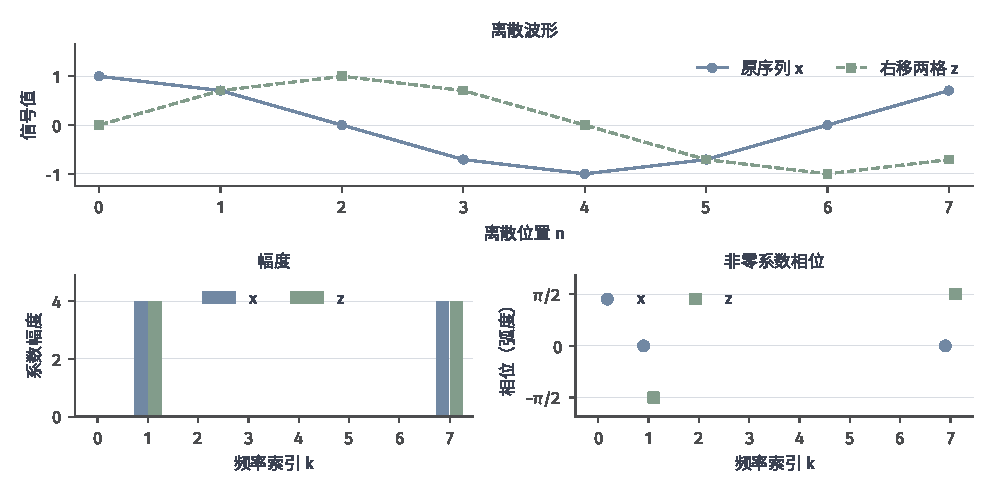
\includegraphics[width=169.0mm]{figures/01-mathematical-preliminaries-upper/03-graphs-and-signals/matplotlib/signal-amplitude-phase/figure.pdf}
  \caption{长度$8$的教学信号$x[n]=\cos(2\pi n/8)$及其循环延迟两格的结果。
  上方波形的峰值位置不同，下方在$k=1,7$的幅度均为$4$，相位却改变。
  相位图只画非零系数；波形连线只帮助观察顺序，不表示已选择连续时间插值。}
  \label{fig:signal-amplitude-phase}
\end{figure*}

这里的复指数坐标来自规则循环平移：每次移动都有统一的方向和步长，DFT同时分解
这些平移。如果位置只通过不规则的连接关联，就不能再根据编号判断谁是“下一格”。
第~\ref{sec:signal-analysis-graph-state-kernels}节将用图上的连接定义变化，
并通过环图说明本节的复指数怎样成为图谱的一个特例。

\subsubsection{周期连续信号的傅里叶表示}

连续时间的一个周期含无穷多个位置，有限个坐标一般不足以完整描述。
周期条件仍把频率限制在整数谐波上，但展开变为无穷级数。
\begin{definition}[周期信号的傅里叶系数与级数]
  \label{def:signal-analysis-fourier-series}
  设$T>0$，$f\in L^2[0,T]$并按周期$T$延拓。在内积
  \[
    \langle f,g\rangle_T=\frac1T\int_0^T f(t)\overline{g(t)}\,\mathrm dt
  \]
  下，复指数$e^{\mathrm i2\pi kt/T}$组成正交归一基。
  \term{傅里叶系数}（Fourier coefficient）为
  \[
    c_k=\frac1T\int_0^T f(t)e^{-\mathrm i2\pi kt/T}\,\mathrm dt,
    \qquad k\in\mathbb Z,
  \]
  相应傅里叶级数写作
  \begin{equation}
    f(t)\sim\sum_{k\in\mathbb Z}c_ke^{\mathrm i2\pi kt/T}.
    \label{eq:signal-analysis-fourier-series}
  \end{equation}
\end{definition}
这里使用周期复指数系在$L^2[0,T]$中完备这一标准结论，其证明不在本节展开。
正交性由对$e^{\mathrm i2\pi(k-j)t/T}$积分得到：$k=j$时归一化积分为$1$，
否则两个端点的指数相同，积分为$0$。完备性给出对称部分和
$S_Kf=\sum_{|k|\leq K}c_ke^{\mathrm i2\pi kt/T}$的$L^2$收敛，
即$T^{-1}\int_0^T|S_Kf-f|^2\to0$。它描述一个周期的平均平方误差，
不能单凭这一结论就在每个$t$写逐点等号。

由正交展开及其极限得到
\begin{equation}
  \frac1T\int_0^T|f(t)|^2\,\mathrm dt
  =\sum_{k\in\mathbb Z}|c_k|^2.
  \label{eq:signal-analysis-continuous-parseval}
\end{equation}
左侧是在一个周期上平均的幅值平方，后面将用它定义周期信号的平均功率。
若计算一个周期的平方积分，还需要乘以$T$；非零周期信号在整条实轴上的平方
积分则为无穷。
相应截断误差为$\sum_{|k|>K}|c_k|^2$。
实信号满足$c_{-k}=\overline{c_k}$，延迟$\tau$则把$c_k$变为
$e^{-\mathrm i2\pi k\tau/T}c_k$，幅相的作用与有限情形相同。

逐点重构需增加规则性。例如在一个周期内分段$C^1$、只有有限个跳跃点且单侧极限
存在时，傅里叶级数在连续点趋于$f(t)$，在跳跃点趋于左右极限平均。
这是带条件的结论；不能把均方收敛与逐点或一致收敛互换，
这些收敛性质的成立条件可回查第~\ref{chap:mathematical-analysis}章。

取周期$2\pi$的方波：$0<t<\pi$时为$1$，$-\pi<t<0$时为$-1$。
平均值$c_0=0$；对$k\neq0$直接积分，
\[
  c_k=\frac1{2\pi}\left(
    \int_0^\pi e^{-\mathrm ikt}\,\mathrm dt
    -\int_{-\pi}^0 e^{-\mathrm ikt}\,\mathrm dt\right)
  =\frac{1-(-1)^k}{\pi\mathrm ik}.
\]
因此偶数$k$的系数为零，奇数$k$的系数为$2/(\pi\mathrm ik)$，也可配对写成
\[
  \frac4\pi\left(\sin t+\frac{\sin3t}{3}+\frac{\sin5t}{5}+\cdots\right).
\]
连续点处恢复$\pm1$，跳跃点处趋于$0$，无论给原函数的跳跃点赋什么值，
其$L^2$元素和傅里叶系数都不变。Parseval仍给出
$1=(8/\pi^2)\sum_{j=0}^{\infty}(2j+1)^{-2}$。
平均平方误差趋零并不排除跳跃附近的局部振荡；这也是有限谐波近似尖锐边沿时
需要单独观察局部误差的原因。

\subsubsection{整轴离散信号的傅里叶表示}

一条整轴序列不必周期，频率也不再局限于$N$个格点。
但整数$n$使$e^{-\mathrm i(\omega+2\pi)n}=e^{-\mathrm i\omega n}$，
因此频率变量虽然连续，频率表示仍以$2\pi$为周期。
\begin{definition}[离散时间傅里叶变换]
  \label{def:signal-analysis-dtft}
  对$x\in\ell_1(\mathbb Z)$，即$\sum_{n\in\mathbb Z}|x[n]|<\infty$的序列，\term{离散时间傅里叶变换}
  （discrete-time Fourier transform, DTFT）定义为
  \begin{equation}
    X(e^{\mathrm i\omega})=\sum_{n\in\mathbb Z}x[n]e^{-\mathrm i\omega n},
    \qquad \omega\in\mathbb R.
    \label{eq:signal-analysis-dtft}
  \end{equation}
  绝对可和使级数绝对且一致收敛，因而定义连续的$2\pi$周期函数。
\end{definition}
记号$X(e^{\mathrm i\omega})$强调只沿单位圆取值，不在这里假设存在一般复变量的
解析延拓。对$x\in\ell_2$，相同级数改按$L^2([-\pi,\pi])$收敛解释，
所得对象是等价类，不要求每个$\omega$都能按普通级数求值。
两种情形均有系数恢复与能量关系
\begin{align*}
  x[n]&=\frac1{2\pi}\int_{-\pi}^{\pi}
  X(e^{\mathrm i\omega})e^{\mathrm i\omega n}\,\mathrm d\omega,\\
  \sum_n|x[n]|^2&=\frac1{2\pi}\int_{-\pi}^{\pi}|X(e^{\mathrm i\omega})|^2\,\mathrm d\omega.
\end{align*}
在$\ell_1$情形可把绝对收敛级数移入积分，单位复指数的正交性留下第$n$项；
$\ell_2$情形则来自周期$L^2$空间的正交基与Parseval关系。

贯穿例零延拓后的DTFT为
$X(e^{\mathrm i\omega})=1+2e^{-\mathrm i\omega}+e^{-2\mathrm i\omega}$，
它是连续频率曲线。对$N\geq3$，将记录补零到$N$项后计算DFT，
只是读取这条曲线在$\omega=2\pi k/N$上的值。补更多零增加了频率格密度，
没有增加原记录的信息或延长真实观测。
相反，若原序列无穷长，先截取$N$项再作DFT，频谱已受时间截断影响，
不能把结果直接称为完整DTFT的精确采样。
离散频率$\omega$的单位是弧度每样本；样本间隔为$T_s$时才换算成
连续角频率$\Omega=\omega/T_s$，并保留模$2\pi/T_s$的歧义。

\subsubsection{整轴连续信号的傅里叶表示}

整条时间实轴既没有有限长度，也不预设周期，复指数坐标随连续频率变化。
求和相应变成积分，但积分存在性与能量空间延拓仍是两种不同依据。
\begin{definition}[连续时间傅里叶变换]
  \label{def:signal-analysis-continuous-fourier-transform}
  对$f\in L^1(\mathbb R)$，连续时间傅里叶变换为
  \[
    F(\Omega)=\int_{\mathbb R}f(t)e^{-\mathrm i\Omega t}\,\mathrm dt.
  \]
  若还满足$F\in L^1$，逆变换
  \[
    f(t)=\frac1{2\pi}\int_{\mathbb R}F(\Omega)e^{\mathrm i\Omega t}\,\mathrm d\Omega
  \]
  在几乎处处意义下成立，右侧给出连续代表元；在原$f$的连续点也恢复其点值。
  在$L^1\cap L^2$上使用同一积分公式，Plancherel定理将变换唯一延拓到$L^2$，
  满足
  \[
    \int_{\mathbb R}|f(t)|^2\,\mathrm dt
    =\frac1{2\pi}\int_{\mathbb R}|F(\Omega)|^2\,\mathrm d\Omega.
  \]
\end{definition}
一般$L^2$情形的正逆变换按范数极限理解，不保证普通积分在每个频率或时刻存在。
例如改变单个点值不会改变$L^2$元素，变换不可能判断这个点后来被赋成哪个值。
第~\ref{sec:signal-bandlimited-recovery}节将借助带限条件选定连续代表元，
然后才读取采样点；不能对任意等价类未经说明直接采样。

一个可直接积分的例子是$f=\mathbb I_{[0,1]}$：
\[
  F(\Omega)=
  \begin{cases}
    (1-e^{-\mathrm i\Omega})/(\mathrm i\Omega),&\Omega\neq0,\\
    1,&\Omega=0.
  \end{cases}
\]
时域函数$f$在$[0,1]$外取零，但频谱$F$在任意大的频率范围外仍可能非零。时间范围
有限因而不能推出频率范围有限。后面采样重构所需的带限条件约束频谱的支撑，
必须另行核对。
对满足积分条件的实信号，$F(-\Omega)=\overline{F(\Omega)}$；
延迟$\tau$使频谱乘上$e^{-\mathrm i\Omega\tau}$，仍只改相位不改幅度。
这里$\Omega$以弧度每单位时间计，不能与DFT的无量纲索引$k$直接比较。

表~\ref{tab:reader-fourier-objects}汇总四种对象。它们的共同点是复指数坐标，
差别来自索引与周期条件，而不是四个名称可以互换。
\begin{table*}[htbp]
  \centering
  \begin{tabularx}{\linewidth}{lXXX}
    \toprule
    表示 & 输入对象及边界 & 频率坐标 & 成立口径\\
    \midrule
    DFT & $N$项数组，基采用循环索引 & $N$个频率格 & 有限和，可逆\\
    傅里叶级数 & 一个周期上的函数 & 全部整数谐波 & $L^2$均方展开；逐点另需条件\\
    DTFT & 整数轴序列，不要求周期 & 连续且$2\pi$周期 & $\ell_1$下连续；$\ell_2$下为$L^2$等价类\\
    连续傅里叶变换 & 实轴函数，不要求周期 & 连续实频率 & $L^1$积分或$L^2$延拓\\
    \bottomrule
  \end{tabularx}
  \caption{信号对象决定傅里叶表示的频率轴及收敛意义。离散时间不表示频率必然离散，
  频谱周期也不表示原序列周期；有限DFT与整轴DTFT还相差记录范围及边界约定。}
  \label{tab:reader-fourier-objects}
\end{table*}

\subsection{有限信号的多项式表示}
\label{sec:signal-analysis-polynomial-arithmetic}

对于有限序列，我们还可以用多项式的幂次记录位置，用系数记录各位置的读数。
由此得到的多项式能够换成点值或余数坐标，不过恢复系数所需的信息量取决于次数界
和选取的坐标。这里先证明什么时候可以恢复，卷积计算中再利用这些表示减少乘法。

\subsubsection{基于位置系数的多项式表示}

对$\bm x=(x_0,\ldots,x_{m-1})$定义
\[
  X(z)=\sum_{j=0}^{m-1}x_jz^j.
\]
其中$x_j=x[j]$，形式变量$z$首先只记录位置，并不是给系统施加的输入。
长度固定后，序列与次数小于$m$的多项式一一对应；最高位置可以是零，
所以次数未必恰好为$m-1$。例如贯穿记录与核分别对应
$X(z)=1+2z+z^2$和$H(z)=1-z$。
移动一个位置并保留前导零对应乘以$z$，而是否把高次项回绕到低次项，
仍要由边界另行规定。正变换DFT正是$X$在单位根$\omega_N^k$处的求值；
多项式在这里连接位置系数与另一组坐标，并未改变记录本身。

\subsubsection{基于互异点值的插值表示}

已知一个多项式在若干位置的值，何时足以恢复全部系数？
答案同时依赖次数界与选点。次数小于$L$的多项式构成$L$维空间。
选取$L$个两两不同的点$a_0,\ldots,a_{L-1}$，求值映射
\[
  E(P)=(P(a_0),\ldots,P(a_{L-1}))
\]
是线性的。若$E(P)=0$，则$P$有$L$个不同根；次数小于$L$的非零多项式
至多有$L-1$个根，因此$P=0$。同维空间间的单射必为双射，
逆映射就是\term{多项式插值}（polynomial interpolation）。

显式恢复可用Lagrange基
\[
  \ell_j(z)=\prod_{\substack{0\leq k<L\\k\neq j}}
  \frac{z-a_k}{a_j-a_k}.
\]
互异性保证分母非零，且$\ell_j(a_k)=\delta_{j,k}$。
故$P$与下式右侧在$L$个点相同、次数都小于$L$，由刚才的唯一性得到
\begin{equation}
  P(z)=\sum_{j=0}^{L-1}P(a_j)\ell_j(z),\qquad\deg P<L.
  \label{eq:signal-analysis-lagrange-interpolation}
\end{equation}
例如一次多项式在$0,1$的值为$1,3$，便恢复为$1(1-z)+3z=1+2z$。
若允许二次项，则$1+2z+c\,z(z-1)$对任意$c$都给出相同两点值，
说明次数界不可省。重复读取同一点也不增加独立约束；导数观测属于另一种插值问题。

代数可逆不等于数值稳定。点值到系数的矩阵逆可能放大测量或舍入误差，
相近选点以及较高次数尤其需要检查条件数，相关判断回用
第~\ref{chap:matrix-analysis}章。单位根的归一化DFT是条件良好的特殊选点，
一般实点并没有同样保证。

\subsubsection{基于互素余数的模分解表示}

点值只保留一个数；有时保留关于低次多项式的余数更方便。
余数记录除掉某个模多项式后还剩下的部分。若模多项式的次数不超过原多项式的次数，
一份余数的次数更低，因而所需的系数更少；多份余数则可能合起来恢复原对象。
为使这种说法有确定含义，先建立除法与唯一性，以下以$F$表示系数域。
域（field）是一套遵守通常加乘运算律、可以加减乘除且非零元素都能作除数的数系；
本节可以先取熟悉的$\mathbb R$或$\mathbb C$。
$F[z]$表示系数在$F$中的有限多项式全体，采用通常的多项式加法与乘法。
\begin{theorem}[多项式带余除法]
  \label{thm:signal-analysis-polynomial-division}
  设$A,M\in F[z]$且$M\neq0$，存在唯一的$Q,R\in F[z]$满足
  \[
    A=QM+R,\qquad\deg R<\deg M.
  \]
  约定零多项式的次数为$-\infty$。
\end{theorem}
\begin{proof}
  若$\deg A<\deg M$，取$Q=0,R=A$。否则设最高次项分别为
  $a_pz^p$与$m_qz^q$，$p\geq q$。域中$m_q$可逆，减去
  $(a_p/m_q)z^{p-q}M$就消掉最高次项。每步次数严格下降，
  有限步后便得到次数小于$\deg M$的余数。

  若还有$A=Q'M+R'$，则$(Q-Q')M=R'-R$。左侧若非零，次数至少为$\deg M$；
  右侧若非零，次数小于$\deg M$，矛盾。因此两侧都为零，$Q=Q'$、$R=R'$。
\end{proof}

对非零$A,B$反复带余除法，
\[
  A=Q_0B+R_1,\qquad B=Q_1R_1+R_2,\qquad\ldots
\]
非零余数的次数严格下降，过程必有限终止。
由$A=Q_0B+R_1$可见，$A,B$的公因式恰好是$B,R_1$的公因式；
逐步应用，最后一个非零除数（包括最初的$B$）首项归一化后就是
\term{最大公因式}（greatest common divisor）。
从最后一个等式向前回代，各余数与初始除数$B$均为$A,B$的多项式线性组合，得到
\begin{equation}
  U(z)A(z)+V(z)B(z)=\gcd(A,B).
  \label{eq:signal-analysis-polynomial-bezout}
\end{equation}
这是Bézout恒等式。互素表示最大公因式为非零常数，等价于存在$U,V$使左侧为$1$。
例如在$\mathbb R[z]$中，
\[
  z^2+1=(z+1)(z-1)+2,\qquad
  1=\tfrac12(z^2+1)-\tfrac12(z+1)(z-1).
\]
它既证明$z-1$与$z^2+1$互素，也提供了后面重构所需的逆元。

把余数记为$A\bmod M$，把相差$M$倍数的多项式看成同一个
\term{剩余类}（residue class），记为$[A]_M$。
当$M=z-a$时，除法式在$z=a$处给出
$A(z)=Q(z)(z-a)+A(a)$，所以点值恰好是关于一次模的常数余数。
下面的\term{多项式中国剩余定理}（polynomial Chinese remainder theorem）说明，互素模下的各份余数怎样共同确定原对象。
\begin{theorem}[多项式中国剩余定理]
  \label{thm:signal-analysis-polynomial-crt}
  设非恒定多项式$m_1,\ldots,m_s\in F[z]$两两互素，令$M=\prod_{j=1}^s m_j$。
  映射
  \[
    [A]_M\longmapsto([A]_{m_1},\ldots,[A]_{m_s})
  \]
  是环同构（ring isomorphism），即双射并且保持加法和乘法；
  余数类相加或相乘，都是先作多项式运算再对相应的模取余。
  因此全部余数唯一确定次数小于$\deg M$的代表元$A\bmod M$。
\end{theorem}
\begin{proof}
  若$A-B$是$M$的倍数，它也是各$m_j$的倍数，故映射不依赖代表元；
  取余还保持加法与乘法。若$A,B$的各个余数都相同，则每个$m_j$整除$A-B$。
  为证明乘积也整除，先设互素的$a,b$均整除$q$，写$q=ac$。
  由$ua+vb=1$有$c=uac+vbc=uq+vbc$，所以$b$整除$c$，从而$ab$整除$q$。
  两两互素时，若某多项式分别与$a,b$互素，将对应Bézout等式相乘即可证明
  它与$ab$互素。反复使用前述整除结论，便有$M\mid(A-B)$，映射为单射。

  给定任意余数$r_j$，令$M_j=M/m_j$。互素性与Bézout恒等式给出
  $u_jM_j+v_jm_j=1$。因此$e_j=u_jM_j$关于$m_j$的余数是$1$，
  关于其他$m_k$的余数是$0$。取
  \[
    A=\sum_{j=1}^s r_je_j
  \]
  即具有全部指定余数，故映射满射。最后对$M$取余，带余除法给出唯一的
  次数小于$\deg M$代表元。
\end{proof}

互素性使各份信息能够独立拼合，次数界使模意义下的唯一性成为原多项式的唯一性。
例如知道$P\bmod z$和$P\bmod(z-1)$可以恢复一次多项式，却无法区分
$P$与$P+c\,z(z-1)$；反复使用同一个模更不增加信息。
在模$z^N-1$下，$z^{N+s}$与$z^s$属于同一剩余类，因而高次系数按模$N$合并。
这个规则将编码循环边界，但此时还没有计算两个信号的乘积。
余数恢复如何减少卷积计算，留到第~\ref{sec:signal-analysis-fast-transforms}节。

\section{信号的比较}
\label{sec:signal-comparison}

不同坐标描述同一条信号，但比较信号还需要确定评价口径。峰值、累计幅值和平方累计
回答不同的大小问题；内积比较模式的方向；长期平均功率则描述持续信号的平均强度。
这些指标都必须针对相同的位置范围与通道单位计算。

\subsection{信号的大小比较}

比较两条记录的大小之前，需要确定比较什么。若约束设备的最大读数，可以看峰值；
若要累计全部幅值，可以求绝对值之和；平方和则让较大的读数占更高权重。
对离散标量信号，这三种口径对应
\[
  \|x\|_\infty=\sup_k|x[k]|,\qquad
  \|x\|_1=\sum_k|x[k]|,\qquad
  \|x\|_2=\left(\sum_k|x[k]|^2\right)^{1/2}.
\]
在有限记录上求和只取记录范围；整轴上则要求相应总和有限。
记$\ell_1(\mathbb Z)$为绝对可和序列空间，$\ell_2(\mathbb Z)$为平方可和序列空间。
例如$x[k]=(k+1)^{-1}$在$k\geq0$时取此值、在$k<0$时取零，
属于$\ell_2$却不属于$\ell_1$。所以可以定义能量的信号未必能直接使用
绝对收敛的变换或卷积论证。

连续情形将和换成积分，得到$L^1$与$L^2$范数；$L^\infty$采用
$\operatorname*{ess\,sup}_t|x(t)|$，即忽略零测异常点后的最小本质上界。
这不同于最大值：函数可能只趋近其上界而未取到，也可能在单个点被赋任意大值，
但代表同一个$L^\infty$元素。真实采样要读取点值，届时必须另行确定代表元。

对贯穿有限记录，$\|x\|_\infty=2$、$\|x\|_1=4$、$\|x\|_2=\sqrt6$。
重排位置不改变这三个数，却可以改变局部波形；范数不是完整的形状描述。
多通道的二范数可按
$\|\bm x\|_2^2=\sum_k\|\bm x[k]\|_2^2$定义，
不同通道若具有不同单位，需要先换算或明确选取权重。下一小节将用带权内积
说明这种比较；这里的欧氏范数约定所有通道已经使用相容的数值尺度。

\subsection{信号的相似性比较}

判断两个记录是否接近，需要决定哪些位置和通道参与比较。
沿用前面说明的第一变量线性约定，对有限记录、平方可和序列与平方可积函数，分别有
\begin{equation}
  \begin{aligned}
    \langle x,z\rangle_N&=\sum_{k=0}^{N-1}x[k]\overline{z[k]},\\
    \langle x,z\rangle_{\ell_2}&=\sum_{k\in\mathbb Z}x[k]\overline{z[k]},\\
    \langle x,z\rangle_{L^2}&=\int_{\mathbb R}x(t)\overline{z(t)}\,\mathrm dt.
  \end{aligned}
  \label{eq:signal-inner-products}
\end{equation}
后两式中的逐点乘积$x[k]\overline{z[k]}$与$x(t)\overline{z(t)}$
由Cauchy--Schwarz不等式分别保证绝对可和与绝对可积。
内积为零表示在当前比较口径下正交，诱导距离为$\|x-z\|_2$。
非零信号的归一化比较量
$\rho(x,z)=\langle x,z\rangle/(\|x\|_2\|z\|_2)$满足$|\rho|\leq1$；
实信号时这是夹角余弦，复信号时它一般是复数，包含相对相位。
零信号没有这种归一化相似性，不能直接除以零。

例如$x=(1,2,1)$、$z=(1,0,-1)$满足$\langle x,z\rangle=0$，
但两者在位置$0$都有非零值。正交描述汇总贡献抵消，不要求支撑互不相交。
若把$x$变成$2x$，归一化相似性仍为$1$，距离却为$\|x\|_2$；
这说明方向相同与数值接近是两个判断。

多通道内积同时汇总位置与通道：
\[
  \langle\bm x,\bm z\rangle
  =\sum_k\sum_{c=1}^d x_c[k]\overline{z_c[k]}.
\]
如果不同传感器的单位或重要性不同，可明确选正权重$w_c$，
把每项乘以$w_c$。更一般地，Hermitian正定矩阵$\bm W$给出
$\sum_k\bm z[k]^*\bm W\bm x[k]$，其中$*$表示共轭转置。
正定性使非零信号的自内积为正；仅半正定时某些非零通道组合可能被忽略。
改变权重可能改变正交关系及相似性排序，不能把它当作不影响结论的单位装饰。

\subsection{信号的能量与功率比较}

振幅和频率都非零的连续时间正弦波可以无限持续。尽管每个时刻的读数有界，
把整条时间实轴上的幅值平方积分，结果仍会发散。此时可以分别研究总累计量和长时间窗口内的
平均累计量，它们对应信号能量与平均功率。
\begin{definition}[信号能量与平均功率]
  \label{def:signal-energy-power}
  离散及连续信号的能量分别为
  \[
    E_x=\sum_{k\in\mathbb Z}|x[k]|^2,\qquad
    E_x=\int_{\mathbb R}|x(t)|^2\,\mathrm dt.
  \]
  能量有限等价于属于相应的$\ell_2$或$L^2$空间，且$E_x=\|x\|_2^2$。
  长期平均功率在相应极限存在时定义为
  \begin{align*}
    P_x&=\lim_{K\to\infty}\frac1{2K+1}\sum_{k=-K}^K|x[k]|^2,\\
    P_x&=\lim_{R\to\infty}\frac1{2R}\int_{-R}^R|x(t)|^2\,\mathrm dt.
  \end{align*}
\end{definition}

这里以幅值平方定义信号指标；若要解释为物理能量或功率，还需相应单位与系统系数。
窗口能量则只在声明的记录窗口求和或积分。
之所以要区分这两者，是因为持续振荡的信号在每个时刻读数有界，累计平方却随
时间线性增长、并不收敛。贯穿例零延拓后的能量为$6$；若将它按周期$3$延拓，
单周期能量仍为$6$，平均功率却为$6/3=2$，而整轴能量发散。
一般周期序列满足$P_x=N^{-1}\sum_{k=0}^{N-1}|x[k]|^2$，
局部平方可积的$T$周期函数满足$P_x=T^{-1}\int_0^T|x(t)|^2\,\mathrm dt$。
两式可由长窗口分成完整周期与长度有界的剩余段得到。

对实参数$A,\Omega,\varphi$且$A\neq0$、$\Omega\neq0$的正弦信号$x(t)=A\cos(\Omega t+\varphi)$，
利用$\cos^2 u=(1+\cos2u)/2$得到一个周期的平方积分为$A^2T/2$，
故$P_x=A^2/2$，而无限多个周期的累计能量为无穷。
相反，有限能量信号的长期平均功率为零，因为平均的分子不超过总能量，
分母却趋于无穷。非周期有界信号未必有平均功率极限，例如按$|t|$把时间轴分成取值$0$和$1$的交替块，
选取各块长度，使此前全部块的总长度与新块长度之比趋于零。沿着各块端点取对称窗口，
平方平均就分别趋近$0$或$1$，因而没有极限。

前面的Parseval关系只是在另一组坐标下计算这里已经定义的能量或周期平均功率。
其中出现$N$、$T$或$2\pi$的尺度因子来自变换与内积的归一化，
不是同一条信号在换坐标后获得了更多能量。

\section{信号的运算与映射}
\label{sec:signal-operations-maps}

时域、频域和多项式坐标已经描述了同一条信号。这些表示讨论的是同一个对象，
接下来要问的是：对信号作一次操作以后，它的各种坐标怎样变化。
平移与反转改变位置，缩放与叠加改变读数或时间尺度；
把这些操作当作系统的输入输出规则后，还要检验系统是否满足线性与平移不变。
三类映射将依次出现：输出只依赖一个位置的无记忆映射，
输出依赖整段历史但仍保持线性与平移不变的卷积映射，
以及权重随输入或时刻改变、因而不满足这两条性质的映射。
模板相关虽然形式上接近卷积，却是把一条信号与不同局部片段比较，
因此单独讨论。每项运算都需要保留前一节约定的边界条件。

\subsection{信号的平移与反转}

为避免对称波形掩盖方向差异，本节固定一个非对称三角脉冲：
\begin{equation}
  x(t)=
  \begin{cases}
    2t,&0\leq t\leq1,\\
    3-t,&1<t\leq3,\\
    0,&\text{其余位置}.
  \end{cases}
  \label{eq:signal-asymmetric-wave}
\end{equation}
它在$t=1$达到峰值$2$，上升历时$1$、下降历时$2$，
能量为$\int_0^1 4t^2\,\mathrm dt+\int_1^3(3-t)^2\,\mathrm dt=4$。
图~\ref{fig:signal-basic-operations}始终用它作参照。

\subsubsection{信号的平移}

连续时间的延迟$\tau$写成$(T_\tau x)(t)=x(t-\tau)$；
离散时间沿用$(T_rx)[k]=x[k-r]$，只允许整数$r$。
正参数使已有特征推迟出现，负参数使其提前。
例如$x(t-1)$的峰值从$t=1$移到$t=2$，支撑从$[0,3]$移到$[1,4]$。
长度$N$的循环延迟则为$x[(k-r)\bmod N]$，越过右端的值回到左端。
对有限非循环记录，必须先按第~\ref{sec:signal-objects-structure}节约定延拓，
再决定是否裁剪到原窗口，不能将丢出窗口的值自动送回首端。

对整轴上同一信号空间的$x,z$，换元给出
$\langle T_\tau x,T_\tau z\rangle=\langle x,z\rangle$；
离散情形用求和换标，循环情形用有限位置的置换得到相同结论。
相应的整轴$L^p$、$\ell_p$范数和能量均不变。
但固定窗口$[0,3]$内，$x(t-1)$只保留原波形的$[0,2]$部分，
窗口能量从$4$降为$11/3$。这是裁剪改变了观测范围，不是平移在整轴上消耗了能量。

\subsubsection{信号的反转}

时间反转定义为$(Rx)(t)=x(-t)$，离散整轴上为$(Rx)[k]=x[-k]$。
它把发生次序沿原点翻转，式~\eqref{eq:signal-asymmetric-wave}的支撑变为$[-3,0]$，
峰值位于$-1$。有限数组通常说的“反序”却是
$x_{\mathrm{rev}}[k]=x[N-1-k]$，$0\leq k<N$；
按整轴零延拓，它等于$T_{N-1}Rx$，是在反转后平移回记录窗口。
循环反转则用$x[(-k)\bmod N]$，位置$0$保持不动，与数组反序也不同。

反转不改变幅值符号；取负$-x(t)$才把正值变成负值，复共轭
$\overline{x(t)}$只改变每个位置的虚部符号。
例如非对称非负波形反转后仍非负，取负后却非正；
复信号$(1+\mathrm i)\mathbb I_{[0,1]}(t)$的共轭仍支持在$[0,1]$，
而时间反转支持在$[-1,0]$，两者不能互换。
换元$t\mapsto-t$或$k\mapsto-k$表明整轴反转保持内积、范数与能量。
后文卷积中的核反转、相关改写中额外的复共轭，将分别使用这里的两项操作。

\subsection{信号的缩放与叠加}

改变幅值和改变时间尺度都可以称为缩放，但两者改变的量不同。前者改变每个位置
的读数，后者重新安排这些读数出现的时刻；相应的能量变化也需分别计算。

\subsubsection{信号的幅值缩放与叠加}

标量倍乘$(ax)(t)=a\,x(t)$改变幅值，逐点相加
$(x+z)(t)=x(t)+z(t)$组合同时位置的值。对任意范数，
$\|ax\|=|a|\|x\|$，故能量为$E_{ax}=|a|^2E_x$；
若长期平均功率存在，也乘以$|a|^2$。
图中的$2x(t)$保持峰值时刻和支撑不变，峰值变为$4$，能量变为$16$，
与把时间压缩一半不是一件事。

叠加时的能量含有干涉项。沿用第一变量线性的内积，
\[
  \|ax+bz\|_2^2
  =|a|^2\|x\|_2^2+|b|^2\|z\|_2^2
   +2\operatorname{Re}\!\left(a\overline b\,\langle x,z\rangle\right).
\]
正交信号的能量直接相加；一般信号可能相互增强或抵消。
有限记录$x=(1,2,1)$与$z=(1,0,-1)$正交，故$\|x+z\|_2^2=6+2=8$；
取$z=x$则$\|x+z\|_2^2=24$而不是$12$，取$z=-x$更会完全抵消。

多通道统一缩放是$a\bm x[k]$，逐通道缩放是对角矩阵$\bm D\bm x[k]$，
一般矩阵$\bm B\bm x[k]$还混合不同通道。
后两种操作不必按同一比例改变总能量；
只有$\bm B^*\bm B=\bm I$时才对所有输入保持欧氏通道能量。
这同时说明“组合两路传感器”必须给出矩阵及通道单位，不能默认为没有损失的重命名。

\subsubsection{信号的时间缩放}

对连续时间信号和实数$a\neq0$，定义$y(t)=x(at)$。
$|a|>1$把时间压缩，$0<|a|<1$把时间伸展，$a<0$还附带时间反转。
若$x$的某个特征位于$t_0$，$y$中的同一特征就位于$t_0/a$。
图中的$x(2t)$峰值仍为$2$，但峰值时刻变为$1/2$，支撑缩短为$[0,3/2]$。
对有限能量信号，换元$s=at$给出
\[
  E_y=\int_{\mathbb R}|x(at)|^2\,\mathrm dt
  =\frac1{|a|}\int_{\mathbb R}|x(s)|^2\,\mathrm ds=\frac{E_x}{|a|}.
\]
因此$x(2t)$的能量为$2$；幅值未变，累计时间却减少。
若需要缩放时间同时保持二范数，应使用$|a|^{1/2}x(at)$。
当平均功率存在时，同样换元并把平均窗口一起缩放，得到$P_y=P_x$，
这与总能量的尺度因子并不矛盾。

整数索引不能随意替换成实数。$x[Mk]$对正整数$M$有定义，表示每$M$项抽取一项；
$x[k/M]$在$k$不是$M$倍数时没有已有样本可读。
插零上采样先规定$u[k]=x[k/M]$在$M\mid k$时成立、其余位置为零，
再由插值规则生成中间值。插零本身不是已经恢复连续波形，抽取也没有
连续时间换元那样的通用能量比例。采样后保留什么信息，须在
第~\ref{sec:signal-analysis-sampling}节另行判断。
\begin{figure*}[htbp]
  \centering
  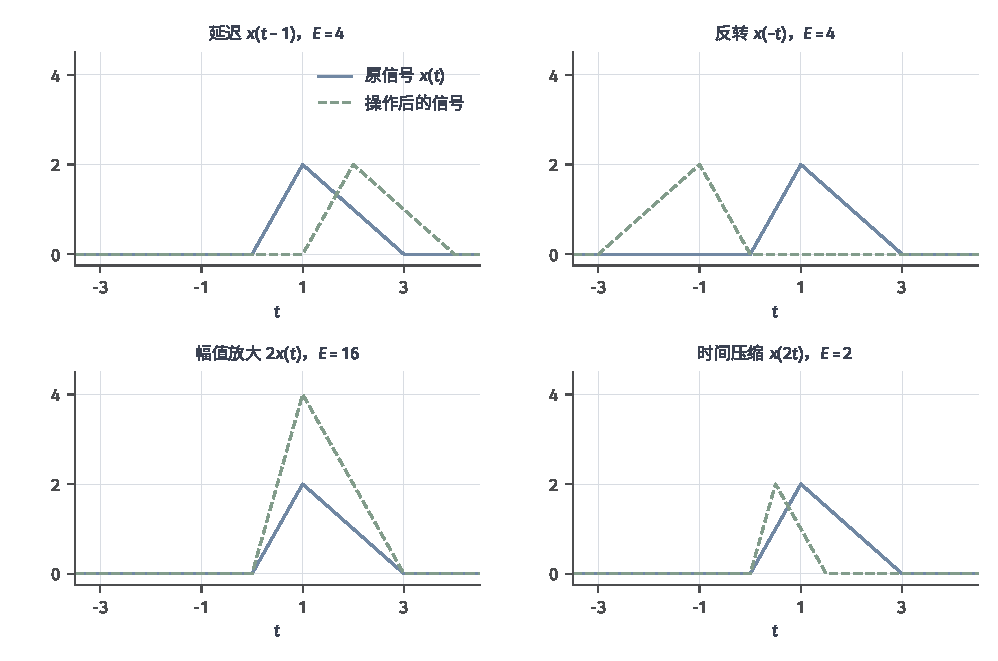
\includegraphics[width=169.0mm]{figures/01-mathematical-preliminaries-upper/03-graphs-and-signals/matplotlib/signal-basic-operations/figure.pdf}
  \caption{对同一非对称三角脉冲分别延迟、反转、放大幅值和压缩时间。
  每幅图的蓝线均为式~\eqref{eq:signal-asymmetric-wave}的原信号，绿线为指定操作结果，
  横轴为时间、纵轴为幅值，坐标尺度一致。平移和反转保持整轴能量$4$，幅值乘$2$使能量变为$16$，
  时间压缩为一半使能量变为$2$；各图均在整轴零值背景下观察，不作窗口裁剪。}
  \label{fig:signal-basic-operations}
\end{figure*}

\subsection{信号之间的映射}
\label{sec:signal-input-output-maps}
\label{sec:signal-analysis-discrete-filtering}

一个系统是把输入信号映为输出信号的规则$y=\mathcal Hx$。
在有限位置上，线性规则可写成$y[n]=\sum_r K[n,r]x[r]$，
其中$K[n,r]$说明位置$r$的单位输入怎样影响位置$n$的输出。
整轴表达还需收敛条件，不能仅凭这个形式就交换无穷求和。
若输入、输出有$d_{\mathrm{in}}$和$d_{\mathrm{out}}$个通道，
则$K[n,r]$应为$d_{\mathrm{out}}\times d_{\mathrm{in}}$矩阵，
矩阵乘法负责混合通道，求和负责汇总时间位置，两者职责不同。

这里的因果性只表示“不读取未来输入”：若两条输入在所有$r\leq n$的位置相同，
则它们在时刻$n$的输出必须相同。对可用脉冲逐项检验的线性核映射，
这等价于$K[n,r]=0$在$r>n$时成立。
输入输出因果性约束读取的时序；干预问题则比较变量机制被指定改变后的响应，
并需要明确干预时保持哪些其他机制不变。相关工具可参考
\BookChapterRef{chap:causal-inference}{卷2《数学准备：概率、因果与决策》第3章“因果响应”}。
只按过去顺序计算一个预测量，不会自动证明其统计关系具有干预含义。

\subsubsection{线性时不变条件下的卷积映射}
\label{sec:signal-analysis-lti-convolution}

设系统已经给出原点处一个单位脉冲的响应。如果其他位置的脉冲只使这条响应相应
平移，而多个脉冲的响应又能按输入幅值相加，我们就能由这一条响应计算全部有限
输入的输出。前一个要求是平移不变，后一个要求是线性，二者分别约束不同的行为。
\begin{definition}[线性时不变系统]
  \label{def:signal-analysis-lti-system}
  设输入、输出信号类为平移封闭的向量空间。若对任意标量$a,b$及输入$x,z$有
  $\mathcal H(ax+bz)=a\mathcal Hx+b\mathcal Hz$，称$\mathcal H$线性。
  若对每个允许的平移量$s$有
  \[
    \mathcal H(T_sx)=T_s(\mathcal Hx),
  \]
  称其具有\term{平移不变性}（shift invariance）。
  离散时间的平移量$s\in\mathbb Z$，连续时间的平移量$s\in\mathbb R$。
  同时满足两者的系统称为线性时不变系统（linear time-invariant system, LTI）。
\end{definition}
这里输入整体移动后输出同样移动，并不是输出保持在原位置。
逐点平方$\mathcal Hx[n]=x[n]^2$平移不变却不线性，
位置加权$\mathcal Hx[n]=n\,x[n]$线性却不平移不变。
是否在每个位置调用了同一段程序，不足以替代这两项等式。

令$h=\mathcal H\delta$，称为\term{脉冲响应}（impulse response）。
有限支撑输入可按式~\eqref{eq:signal-analysis-impulse-expansion}作有限展开，
线性性与平移不变性给出
\begin{align}
  (\mathcal Hx)[n]
  &=\mathcal H\left(\sum_r x[r]T_r\delta\right)[n]\notag\\
  &=\sum_r x[r](T_rh)[n]=\sum_r x[r]h[n-r].
  \label{eq:signal-analysis-lti-convolution}
\end{align}
它把各位置输入所触发的响应相加。
对$x\in\ell_1(\mathbb Z)$，还需
$\mathcal H:\ell_1\to\ell_1$为有界线性且平移不变的算子，
即存在常数$C$使$\|\mathcal Hx\|_1\leq C\|x\|_1$。
令$x^{(K)}=\sum_{|r|\leq K}x[r]T_r\delta$，则$x^{(K)}\to x$于$\ell_1$，
有界性使$\mathcal Hx^{(K)}\to\mathcal Hx$。同时$h=\mathcal H\delta\in\ell_1$，
且
\[
  \sum_n\sum_r|x[r]h[n-r]|=\|x\|_1\|h\|_1<\infty.
\]
因此卷积和绝对收敛，有限截断的卷积也在$\ell_1$中趋于该和，
从而式~\eqref{eq:signal-analysis-lti-convolution}延伸到全部$\ell_1$输入。
不能省略连续性，直接把仅对有限和成立的代数线性搬进无穷和。

这种求和称为\term{离散卷积}（discrete convolution），规则网格上也可用同一结构。
\begin{definition}[网格上的离散卷积]
  \label{def:signal-analysis-discrete-convolution}
  对$x,h\in\ell_1(\mathbb Z^d)$，定义
  \begin{equation}
    (x*h)[\bm n]=\sum_{\bm r\in\mathbb Z^d}x[\bm r]h[\bm n-\bm r].
    \label{eq:signal-analysis-discrete-multidimensional-convolution}
  \end{equation}
  这里$\bm n,\bm r$为网格位置，$h$称为\term{卷积核}（convolution kernel）。
  各位置的和绝对收敛，输出仍属于$\ell_1(\mathbb Z^d)$。
\end{definition}
存在性可直接检查：对非负项换序并令$\bm s=\bm n-\bm r$，有
\[
  \sum_{\bm n}\sum_{\bm r}|x[\bm r]h[\bm n-\bm r]|
  =\left(\sum_{\bm r}|x[\bm r]|\right)
   \left(\sum_{\bm s}|h[\bm s]|\right)<\infty.
\]
所以每个内层和均有限，并得到
$\|x*h\|_1\leq\|x\|_1\|h\|_1$。
核为有限支撑时，对任何逐点有限的输入也可作有限和，但输出不因此必属$\ell_1$。
一维记法为
\begin{equation}
  (x*h)[n]=\sum_{r\in\mathbb Z}x[r]h[n-r].
  \label{eq:signal-analysis-linear-convolution}
\end{equation}
固定$n$后，$r$增加时核索引$n-r$减小，这就是核的反向读取。
令$s=n-r$可得$(x*h)[n]=\sum_s h[s]x[n-s]=(h*x)[n]$，故有交换律；
绝对可和等允许换序的条件还给出结合律和分配律。
若$h[r]=0$对所有$r<0$成立，则$y[n]=\sum_r h[r]x[n-r]$只用当前及过去输入，
系统因果；一般LTI则不必因果，例如三点中心均值会使用$x[n+1]$。

离散卷积逐位置求和。连续时间没有可逐个枚举的位置，因此要用积分累计输入
与平移核的乘积，并先确认该积分确实定义了一个可积输出。
\begin{definition}[连续卷积]
  \label{def:signal-analysis-continuous-convolution}
  设$f,g\in L^1(\mathbb R^d)$，定义
  \begin{equation}
    (f*g)(\bm t)=\int_{\mathbb R^d}f(\bm\tau)g(\bm t-\bm\tau)\,\mathrm d\bm\tau.
    \label{eq:signal-analysis-continuous-convolution}
  \end{equation}
  积分对几乎处处的$\bm t$绝对收敛，并定义$L^1(\mathbb R^d)$中的元素。
\end{definition}
由定理~\ref{thm:analysis-tonelli-fubini}，对非负函数换序并平移换元，
\[
  \int_{\mathbb R^d}\int_{\mathbb R^d}
  |f(\bm\tau)g(\bm t-\bm\tau)|\,\mathrm d\bm\tau\,\mathrm d\bm t
  =\|f\|_{L^1}\|g\|_{L^1}<\infty.
\]
内层积分因而几乎处处有限，且$\|f*g\|_{L^1}\leq\|f\|_{L^1}\|g\|_{L^1}$。
换元和换序同样给出交换律、结合律，但$L^1$假设不保证每个指定点的积分都有限。
这里定义的是两个普通可积函数的卷积，并非所有连续时间LTI算子都具有普通$L^1$核。
例如恒等映射是LTI，它的单位脉冲响应可用Dirac分布（Dirac distribution）
$\delta_0$描述。这里“分布”采用广义函数的用语：这个对象作用于光滑紧支撑的
测试函数$\phi$时返回$\delta_0(\phi)=\phi(0)$，也就是零点单位质量对$\phi$的积分。
对光滑紧支撑的$f$，卷积让它读取$\tau\mapsto f(t-\tau)$在零点的值，
于是$(f*\delta_0)(t)=f(t)$，正好实现恒等映射。
普通函数$\mathbb I_{\{0\}}$的Lebesgue积分却为零，不能承担这种单位质量，
所以不能把离散$\delta[k]$直接当作连续可积核。
当前不调用一般分布理论来证明所有连续系统的核表示。

\begin{example}[区间重叠产生三角形响应]
  \label{ex:signal-analysis-continuous-overlap}
  取$f(t)=g(t)=\mathbb I_{[0,1]}(t)$。两因子同时为$1$要求
  $\tau\in[0,1]\cap[t-1,t]$，因此
  \[
    (f*g)(t)=
    \begin{cases}
      t,&0\leq t\leq1,\\
      2-t,&1<t\leq2,\\
      0,&\text{其余位置}.
    \end{cases}
  \]
  输出先随重叠长度增大而上升，再随重叠减小而下降。
  二维指示函数的相应积分计算重叠面积，一般带符号核则计算加权贡献，
  不能都解释为几何大小。
\end{example}
图~\ref{fig:reader-continuous-convolution-overlap}区分输出位置$t$和积分变量$\tau$。
三角形输出不是把两个输入图形相加，而是把每个$t$处的重叠长度汇成曲线。
\begin{figure*}[htbp]
  \centering
  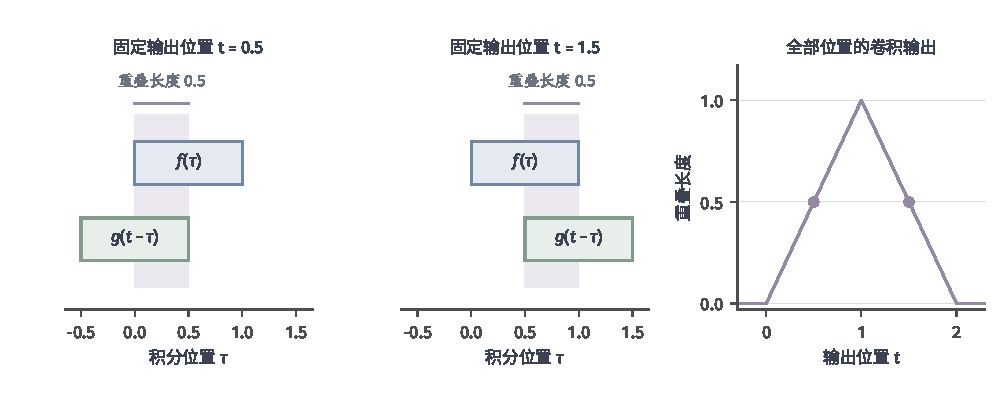
\includegraphics[width=169.0mm]{figures/01-mathematical-preliminaries-upper/03-graphs-and-signals/matplotlib/reader-continuous-convolution-overlap/figure.pdf}
  \caption{教学函数$f=g=\mathbb I_{[0,1]}$的连续卷积。左两图分别固定$t=0.5$与$t=1.5$，
  蓝色为$f(\tau)$的支撑，绿色为$g(t-\tau)$的支撑，紫色重叠区间的长度均为$0.5$。
  右图汇总全部$t$处的重叠长度，在$t=1$时达到$1$。
  左图横轴$\tau$用于积分，右图横轴$t$标记输出位置。}
  \label{fig:reader-continuous-convolution-overlap}
\end{figure*}

回到有限输入。若$x,h$的支撑分别为$0,\ldots,m-1$和$0,\ldots,r-1$，
零延拓线性卷积只可能在$0,\ldots,m+r-2$非零，完整输出长度为$m+r-1$。
贯穿例逐项为
\begin{align*}
  (x*h)[0]&=1,\\
  (x*h)[1]&=2-1=1,\\
  (x*h)[2]&=1-2=-1,\\
  (x*h)[3]&=-1.
\end{align*}
即
\begin{equation}
  \bm x*\bm h=(1,1,-1,-1).
  \label{eq:signal-analysis-running-linear-convolution}
\end{equation}
这个核计算当前值减去前一个值，首尾还包含零延拓带来的跳变。
特别是第一项之前补的是$0$，所以首项为$1-0=1$。
长度$N$的循环索引则在一个周期内求和：
\begin{equation}
  (x*_Nh)[n]=\sum_{r=0}^{N-1}x[r]h[(n-r)\bmod N],
  \qquad n=0,\ldots,N-1.
  \label{eq:signal-analysis-circular-convolution}
\end{equation}
\begin{definition}[循环卷积]
  \label{def:signal-analysis-circular-convolution}
  对长度$N$的实或复序列，式~\eqref{eq:signal-analysis-circular-convolution}
  定义其\term{循环卷积}（circular convolution），输出仍有$N$项。
  它在有限循环索引集上求和，不是两条周期延拓序列在整数轴上的无穷卷积。
\end{definition}
把$h$补成$(1,-1,0)$并取$N=3$，得到$x*_3h=(0,1,-1)$。
此时第一项的前一个值是记录末项$1$，所以首项变为$1-1=0$。
完整线性卷积的末项$-1$回绕到首项，与$1$相消；不是直接删掉了末项。
若对两条周期序列在整轴无穷求和，同一贡献会被重复无穷次。
这里改变的是窗口外怎样连接。FFT只能加速已经选定的映射，不能决定首尾应该怎样连接；
若要用循环计算得到四项完整线性输出，必须补零到足以容纳这四项，避免回绕。
图~\ref{fig:signal-convolution-boundaries}对比零延拓与循环边界下的输出。
\begin{figure}[!htb]
  \centering
  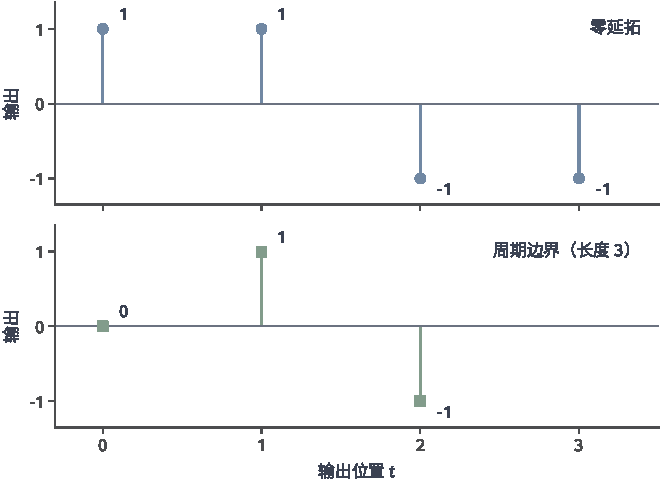
\includegraphics[width=112.0mm]{figures/01-mathematical-preliminaries-upper/03-graphs-and-signals/matplotlib/signal-convolution-boundaries/figure.pdf}
  \caption{输入$(1,2,1)$与核$(1,-1)$的边界比较。蓝色圆点采用零延拓，给出四项线性卷积；
  绿色方点采用长度$3$的循环边界，末项$-1$回到首项并与$1$抵消。
  竖线连接零基线与各离散输出，不定义整数之间的信号值。}
  \label{fig:signal-convolution-boundaries}
\end{figure}

固定输入输出位置后，线性卷积是Toeplitz矩阵乘法，循环卷积是循环矩阵乘法。
例如同一个贯穿例给出
\begin{gather*}
  \begin{bmatrix}
    1&0&0\\-1&1&0\\0&-1&1\\0&0&-1
  \end{bmatrix}
  \begin{bmatrix}1\\2\\1\end{bmatrix}
  =\begin{bmatrix}1\\1\\-1\\-1\end{bmatrix},\\
  \begin{bmatrix}1&0&-1\\-1&1&0\\0&-1&1\end{bmatrix}
  \begin{bmatrix}1\\2\\1\end{bmatrix}
  =\begin{bmatrix}0\\1\\-1\end{bmatrix}.
\end{gather*}
重复对角线反映参数共享，边界则改变矩阵首尾行。
无限网格或循环群上的平移不变性是精确的；有限区间采用零填充、反射或截取后，
通常不再具有同一意义的全局平移不变性。

“valid”只选择核完全落在已知输入内的输出。
按$h[0],\ldots,h[r-1]$的因果索引，当$m\geq r$时保留$n=r-1,\ldots,m-1$，
共$m-r+1$项；$m<r$时没有这样的输出。
保持输入长度的“same”还需指定左右填充及截取位置，不能只凭名称确定。
表~\ref{tab:signal-boundary-conventions}将延拓和输出选择分开，
后文FFT也必须遵守同一约定。
\begin{table*}[!htb]
  \centering
  \begin{tabularx}{\linewidth}{lXXX}
    \toprule
    约定 & 区间外输入 & 保留输出 & 贯穿例\\
    \midrule
    完整线性卷积 & 零延拓 & $0,\ldots,m+r-2$ & $(1,1,-1,-1)$\\
    有效区间选段 & 不使用区间外值 & $r-1,\ldots,m-1$，$m\geq r$ & $(1,-1)$\\
    $N$点循环卷积 & 周期边界 & $0,\ldots,N-1$ & $N=3$时$(0,1,-1)$\\
    \bottomrule
  \end{tabularx}
  \caption{边界延拓与输出选段。$m$为输入长度，$r$为核长度，使用本章因果核索引。
  有效选段不是另一种卷积定义，循环边界也不是零边界的近似。}
  \label{tab:signal-boundary-conventions}
\end{table*}

有了有限DFT，循环卷积可在频率坐标中逐项计算。
\begin{theorem}[离散循环卷积定理]
  \label{thm:signal-analysis-circular-convolution-theorem}
  设$x,h$为长度$N$的复序列，采用式~\eqref{eq:signal-analysis-dft}的约定，则
  \[
    \widehat{x*_Nh}[k]=\widehat x[k]\widehat h[k],\qquad k=0,\ldots,N-1.
  \]
\end{theorem}
\begin{proof}
  令$a=(n-r)\bmod N$，直接换有限求和的索引，
  \begin{align*}
    \widehat{x*_Nh}[k]
    &=\sum_{n=0}^{N-1}\sum_{r=0}^{N-1}
      x[r]h[(n-r)\bmod N]\omega_N^{kn}\\
    &=\sum_{r=0}^{N-1}\sum_{a=0}^{N-1}
      x[r]h[a]\omega_N^{k(r+a)}\\
    &=\left(\sum_{r=0}^{N-1}x[r]\omega_N^{kr}\right)
      \left(\sum_{a=0}^{N-1}h[a]\omega_N^{ka}\right).
  \end{align*}
  固定$r$后，$n$遍历一个周期使$a$也恰遍历一个周期。
  即使$n$与$r+a$相差$N$的整数倍，$\omega_N^{kN}=1$仍使指数相同。
  最后两项分别为$\widehat x[k]$与$\widehat h[k]$。
\end{proof}
于是
\begin{equation}
  x*_Nh=\mathcal F_N^{-1}\bigl(\mathcal F_N(x)\odot\mathcal F_N(h)\bigr).
  \label{eq:signal-analysis-frequency-domain-convolution}
\end{equation}
\BookEquationAliases{\label{eq:cnn-fft-convolution}
\label{eq:cnn-convolution-theorem-derivation}}
若$\bm C_h$为循环卷积矩阵，定理对所有$x$成立，故
$\bm F\bm C_h=\operatorname{diag}(\widehat{\bm h})\bm F$，从而
$\bm C_h=\bm F^{-1}\operatorname{diag}(\widehat{\bm h})\bm F$。
这完整说明DFT如何对角化循环卷积：核的DFT系数是各频率模式的特征值。
要用它得到完整线性卷积，两个输入均须补零到
\begin{equation}
  N\geq m+r-1.
  \label{eq:signal-analysis-linear-padding-condition}
\end{equation}
因为所有非零输出索引此时都小于$N$，不会回绕。
$N\geq\max(m,r)$只保证装下输入，不保证装下输出。

整轴频率响应改用DTFT。若$h\in\ell_1$或具有有限支撑，
即使复指数$x[n]=e^{\mathrm i\omega n}$自身不在$\ell_1$中，仍有绝对收敛的和
\[
  (x*h)[n]=\sum_r h[r]e^{\mathrm i\omega(n-r)}
  =e^{\mathrm i\omega n}\sum_r h[r]e^{-\mathrm i\omega r}.
\]
输出保持频率，只乘以
\begin{equation}
  H(e^{\mathrm i\omega})=\sum_r h[r]e^{-\mathrm i\omega r},
  \label{eq:signal-analysis-filter-frequency-response}
\end{equation}
即\term{频率响应}（frequency response）。模长给出放大或衰减，相角给出该模式的
相位变化；除非相位随频率具有相应线性形式，不能将所有频率的相位变化都叫同一时间延迟。
对$x,h\in\ell_1$，绝对可和允许换序，直接得到
$Y(e^{\mathrm i\omega})=X(e^{\mathrm i\omega})H(e^{\mathrm i\omega})$。
同理，连续$L^1$卷积的傅里叶变换为$F(\Omega)G(\Omega)$，
其积分换序由前面的绝对积分界保证。

贯穿核的响应为$H(e^{\mathrm i\omega})=1-e^{-\mathrm i\omega}$，
模长为$2|\sin(\omega/2)|$。在主频率区间$|\omega|\leq\pi$内，
模长随$|\omega|$从$0$到$\pi$增大：常量模式被消去，低频缓变被削弱，
较高频的差异更突出。这一比较按模$2\pi$重复，不能沿整个实频率轴作单调解释；
有限输入首尾仍受延拓影响。

多通道卷积将标量核换成矩阵核：
\begin{equation}
  y_a[n]=\sum_{b=1}^{d_{\mathrm{in}}}\sum_{r\in\mathbb Z}
  H_{a,b}[r]x_b[n-r],
  \qquad a=1,\ldots,d_{\mathrm{out}}.
  \label{eq:signal-multichannel-convolution}
\end{equation}
各$H_{a,b}\in\ell_1$、各$x_b\in\ell_1$时，有限通道求和与前述界保证存在性；
有限核则在每个位置作有限计算。相同输入输出通道数且$\bm H[r]$总是对角矩阵时，
各通道分别滤波而不混合；非对角元素允许输入通道$b$影响输出通道$a$。
记$\bm X(e^{\mathrm i\omega})$与$\bm Y(e^{\mathrm i\omega})$为各通道DTFT组成的向量，
$\bm H(e^{\mathrm i\omega})$的第$(a,b)$项为核$H_{a,b}$的DTFT，则整轴频域关系为
$\bm Y(e^{\mathrm i\omega})=\bm H(e^{\mathrm i\omega})\bm X(e^{\mathrm i\omega})$。
每个频率上是矩阵乘向量，不是把所有通道分别做一个标量乘法。

无时间记忆的特例$\bm H[0]=\bm B$、其余为零，只在同一时刻混合通道。
取式~\eqref{eq:signal-multichannel-record}中的记录及
$\bm B=\begin{bmatrix}1&1\\1&-1\end{bmatrix}$，有
\[
  \bm Y=\bm X\bm B^\top
  =\begin{bmatrix}1&1\\3&1\\3&-1\end{bmatrix}.
\]
如图~\ref{fig:signal-channel-mixing}所示，输出第一通道为和，第二通道为差，
三个时间位置未变。总能量从$11$变为$22$，因为$\bm B^\top\bm B=2\bm I$；
用$\bm B/\sqrt2$才保持能量。混合前若两路未按时间对齐，矩阵计算本身不会修正偏移。
\begin{figure*}[htbp]
  \centering
  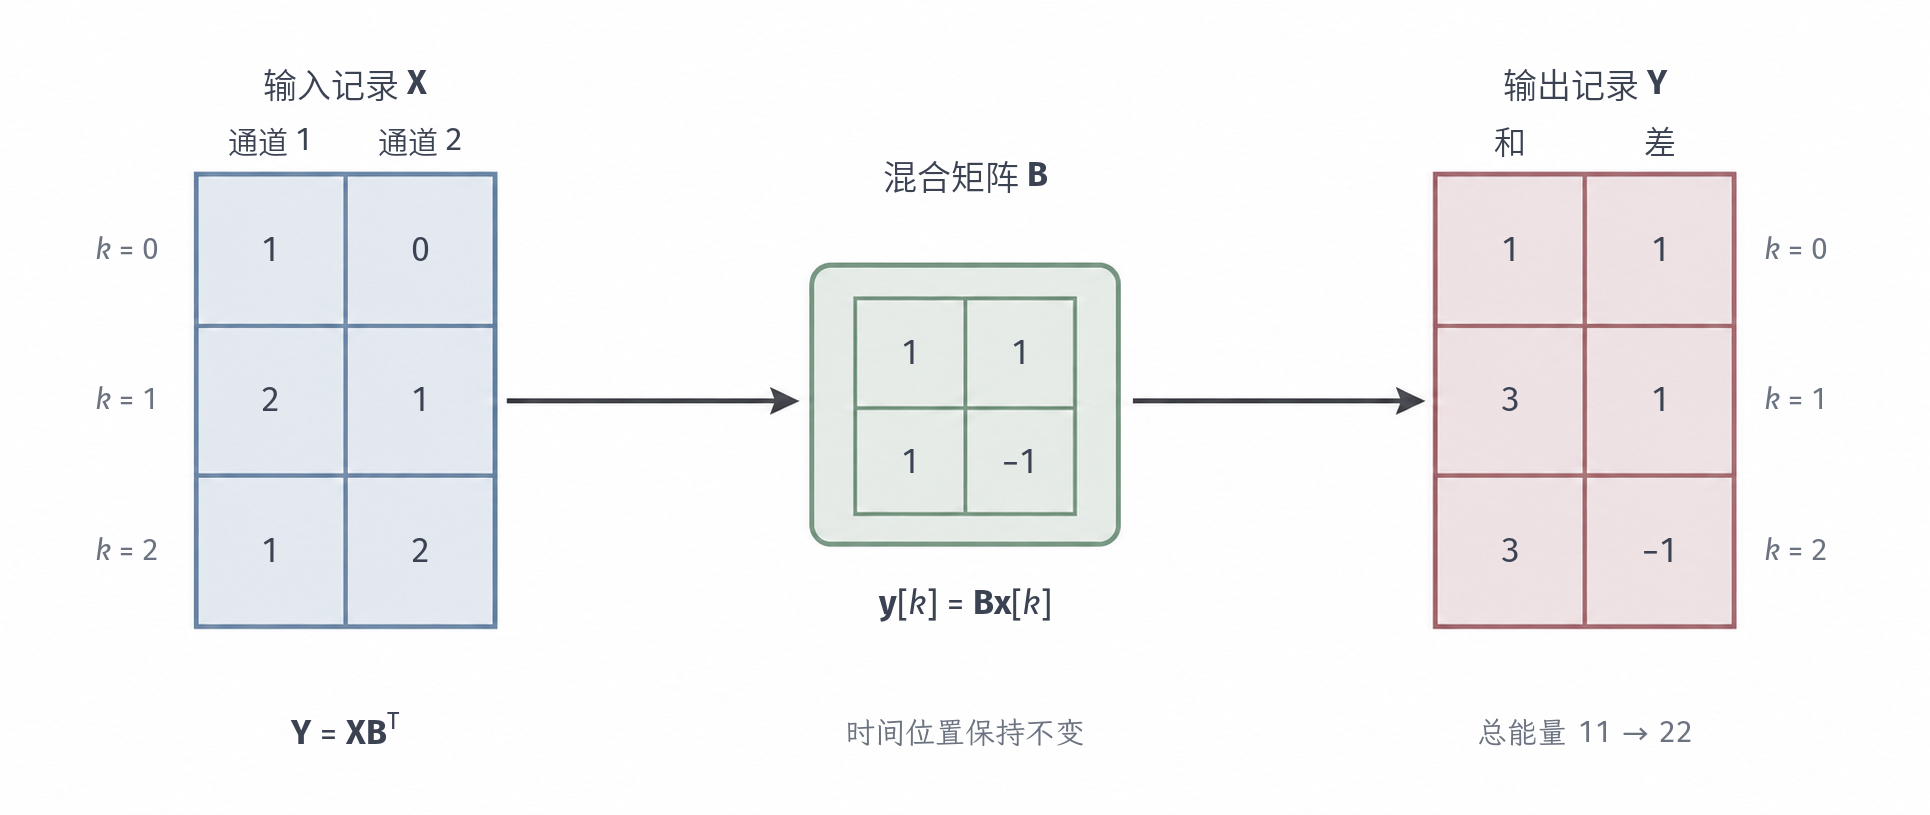
\includegraphics[width=168.998mm]{figures/01-mathematical-preliminaries-upper/03-graphs-and-signals/generated/signal-channel-mixing/figure.png}
  \caption{同一双通道三时刻记录的轴与混合。左侧行标记时间、列标记通道；
  中间矩阵$\bm B$对每一行对应的同时读数取和与差，右侧时间轴长度仍为$3$。
  通道混合不是时间平移，也不意味着两个输入通道独立；这里只使用当前时刻的值。}
  \label{fig:signal-channel-mixing}
\end{figure*}

\subsubsection{线性时变条件下的历史映射}

设备增益随时刻变化时，同样的脉冲在不同时间可能触发不同响应，线性却仍可成立。
用已给定的两时刻核表示
\begin{equation}
  \bm y[n]=\sum_{r\leq n}\bm K[n,r]\bm x[r].
  \label{eq:signal-given-time-varying-kernel}
\end{equation}
有限历史窗口中它是有限和；无限历史中则需另行保证收敛，
例如对有界输入可要求$\sum_{r\leq n}\|\bm K[n,r]\|<\infty$。
求和只取$r\leq n$规定因果性，矩阵维度仍为
$d_{\mathrm{out}}\times d_{\mathrm{in}}$。
核事先固定、不随输入改变时，该表达满足叠加。
若同时满足$\bm K[n+s,r+s]=\bm K[n,r]$，才只依赖滞后$n-r$，
并可记成固定卷积核；只因它累加历史，不能省掉这项条件。

例如令$a[n]$在偶数时为$1$、奇数时为$2$，
$y[n]=a[n](x[n]+\tfrac12x[n-1])$。
它的两时刻核仅在$r=n,n-1$非零，且取值随绝对时刻$n$变化。
输入$\delta[n]$在时刻$0$给出$1$，将输入延迟一格后，时刻$1$的输出却为$2$，
而原输出延迟一格在该处仍为$1$，因此不平移不变。
相反，事先给定$h[0]=0$、$h[r]=2^{-(r-1)}$（$r\geq1$）及负索引为零，
就定义了一个有衰减记忆的固定卷积核。对零延拓$x=(1,2,1)$，
从时刻$0$起的前四项输出为$(0,1,5/2,9/4)$，每次使用相同的滞后权重。

这些例子通过给定核计算输入输出。内部状态演化也能产生固定核与两时刻核，
但构造时需要区分初始状态的自由响应、当前输入的直接项和输入驱动项。
状态演化中的有序矩阵乘积解释核从何而来，本节先检验给定核定义的映射。
若另加一个与输入无关且非零的自由响应，总映射一般是仿射而非线性，
不能仅因输入驱动部分线性就忽略这一差别。

\subsubsection{非线性条件下的输入输出映射}

前面的历史核在输入变化时保持固定。若权重由输入本身决定，输出仍可写成加权
形式，但检验线性时必须连同权重的变化一起计算。一个更简单的非线性例子是$(\mathcal Hx)[n]=x[n]^2$：对$x[n]=1$，
$\mathcal H(2x)[n]=4\neq2\mathcal Hx[n]$，故不线性。
但$\mathcal H(T_rx)[n]=x[n-r]^2=T_r(\mathcal Hx)[n]$，所以它仍平移不变，
且只使用当前值，满足这里的因果性。

再看输入依赖门控
\[
  y[n]=g(x[n])x[n],\qquad g(v)=\frac1{1+e^{-v}}
\]
（此例取实数输入）。门控是由当前输入决定的权重。
记标量响应为$\varphi(v)=g(v)v$。输入$1$与$2$得到的比例分别是$g(1)$与$g(2)$，两者不同，
所以$\varphi(2)\neq2\varphi(1)$；固定同一时刻把输入加倍，输出没有按相同比例变化。
尽管每个位置使用同一规则，叠加仍不成立。
更一般的$\sum_{r\leq n}K_x[n,r]x[r]$既要检查核如何依赖输入，
也要检查计算$K_x$时是否依赖未来输入值。求和表面上只到$n$，
不代表输入依赖的权重一定因果。

可微映射在固定输入附近可以线性化。先在每个位置考察平方这一标量映射，它满足
$(x_0+\varepsilon v)^2=x_0^2+2\varepsilon x_0v+\varepsilon^2v^2$，
一阶响应是$v\mapsto2x_0v$。它依赖展开位置$x_0$，只描述小扰动；
不能据此给全部输入配同一个频率响应。
状态参数若由输入选择，也须连同它们对输入的响应一起检验叠加，
不能把固定输入附近的线性化当作全局固定核。

\subsection{信号的相关运算}
\label{sec:signal-template-correlation}

卷积叠加输入激起的响应；寻找某个波形出现在哪里，则更自然地把模板与不同片段作内积。
采用本章方向约定，\term{互相关}（cross-correlation）为
\begin{equation}
  (x\star h)[n]=\sum_{r\in\mathbb Z}x[n+r]\overline{h[r]}.
  \label{eq:signal-analysis-cross-correlation}
\end{equation}
固定$n$后，比较的是片段$r\mapsto x[n+r]$与原方向模板$r\mapsto h[r]$；
第二个变量取共轭，与前面的内积约定一致。
若$x,h\in\ell_2$，Cauchy--Schwarz保证每个$n$处绝对收敛；
有限模板则只需对应片段逐点有定义。

令$\widetilde h[r]=\overline{h[-r]}$，换元可得
\[
  (x*\widetilde h)[n]=\sum_s x[s]\overline{h[s-n]}
  =\sum_r x[n+r]\overline{h[r]}=(x\star h)[n].
\]
所以相关可以用共轭反转核的卷积实现，模板自身却按原方向比较。
多通道模板在同一$n$处按已声明的通道内积汇总：
$\sum_r\sum_c x_c[n+r]\overline{h_c[r]}$，
带权版本为$\sum_r\bm h[r]^*\bm W\bm x[n+r]$。
若归一化，应同时使用当前片段与模板的非零范数，窗口或权重变化也会改变相似性。

仍取零延拓$x=(1,2,1)$、$h=(1,-1)$。
模板完全在输入内时，相关在$n=0,1$得到$1-2=-1$与$2-1=1$；
完整相关在$n=-1,0,1,2$依次为$(-1,-1,1,1)$。
完整卷积则在$n=0,1,2,3$得到$(1,1,-1,-1)$，
而valid卷积在$n=1,2$给出$(1,-1)$。
差异既来自核方向，也来自输出索引，不能只看数组长度判断二者相同。
许多神经网络库把不反转实核的相关称为“卷积”，训练参数可适应该约定；
手算、复用核或推导伴随算子时，仍须明确反转、共轭、延拓及输出范围。

\section{卷积映射的快速计算}
\label{sec:signal-analysis-fast-transforms}

\subsection{局部汇总的代价与五条计算路线}

上一节说明，线性且平移不变的映射由一条脉冲响应$h$完全决定，输出是输入与$h$的卷积。
这个结论把“设计一个系统”化简成“设计一个核”，但它同时留下一个计算问题：
给定输入和核，怎样求出输出。这个问题的规模由数据本身决定，
一段一分钟的音频在两万赫兹采样下有一百二十万个样本，
一张中等大小的图像有数百万像素，而图像滤波往往要在许多通道、许多核上重复同样的局部点积。
按定义直接求和，每个输出位置要读遍核覆盖的全部输入，总乘加量与“输出位置数×核元素数”成正比。
在常见设置下这个量级可以达到十亿次以上，因此需要寻找复用了中间结果、或者用更少乘法完成同样任务的算法。

卷积之所以值得单独研究，不只因为它描述LTI系统。许多机器学习操作在形式上就是局部加权汇总：
图像上的平滑与边缘检测把每个像素邻域的亮度按核权重加起来；
一维序列上的移动平均用相邻若干项的加权和替换当前值；
处理序列的模型沿时间轴累积历史信息时，也大量使用这类按滞后加权的线性组合。
这些操作的共同结构是输出某一点的取值只取决于输入在一个固定大小窗口内的值，
窗口逐点平移而权重不变。核与输入位置无关，这正是本章要利用的性质：
一旦同一个小窗口反复出现，就有可能只算一次它的贡献，让多个输出共用。

不过“共用”不是无条件成立的，它取决于所求的输出范围。
按定义直接求完整线性卷积时，会枚举核元素与输入元素的全部配对乘积；
只求一个valid输出块时，这种直接算法可以略去不参与所需输出的乘积。
不过这些是直接算法的工作量，不是任何算法都必须逐项支付的代价；
后面的求值与插值正是为了不单独计算每个原始乘积，仍恢复完整结果。
若索引本身是循环的，
答案又变成循环卷积。三种目标的多项式表示不同，可用的加速手段也不同。
因此下面的比较都固定同一组输入和核，只在计算过程上作改变，
避免把“换了目标”误当成“换了算法”。

\begin{table*}[htbp]
  \centering
  \begin{tabularx}{\linewidth}{@{}lXXX@{}}
    \toprule
    路线 & 朴素做法贵在哪里 & 改变的环节 & 代价出现在哪里\\
    \midrule
    直接求和 & 每个输出重算该窗口的全部乘积 & 无 & 乘加量随核元素数线性增长\\
    矩阵化 & 大量短点积逐个调用底层例程 & 只改变计算的组织形式 & 普通矩阵乘法不减少乘加，只是让库函数能统一优化\\
    FFT & 每个频率都要逐个积求和 & 改用频率坐标，把卷积变成逐点乘法 & 需要补零、复数运算与正反变换\\
    Toom--Cook & 全部乘积都当独立的乘法 & 用求值与插值替代高次系数乘法 & 增加求值、插值与常数除法，且会算出不需要的系数\\
    Winograd & 为每个输出重复同一套点积 & 固定小窗口的变换，只用一次小块乘法 & 变换矩阵的尺度差异会放大舍入误差\\
    空间可分离 & 二维核的乘法量是两轴长度之积 & 把二维核写成两个一维核的组合 & 只有核具有相应低秩结构时才成立\\
    \bottomrule
  \end{tabularx}
  \caption{同一卷积目标下五条计算路线的改动位置。每一条都回答“原来的哪一步贵”，
  因此它们可以在同一份输入上比较；选择哪一条还要结合核的大小、输出范围和数值精度要求。
  表中列出的是改动环节，不承诺某条路线在任意规模下都更快。}
  \label{tab:signal-analysis-fast-transform-roadmap}
\end{table*}

把卷积写成多项式乘法是上述比较的统一语言。多项式只是把数组的第$j$个位置记成幂次$z^j$、
把读数记成系数，并不引入新的数据，但它让“按位置汇总”变成了“按幂次合并同类项”，
后文的取余、求值和插值都作用在这个多项式上。

先固定所求的是完整线性卷积、循环卷积，还是某个valid输出块，再比较计算路线。
对有限序列的多项式$X(z)=\sum_{i=0}^{m-1}x_i z^i$与
$H(z)=\sum_{j=0}^{r-1}h_jz^j$，乘积为
\begin{align}
  X(z)H(z)
  &=\sum_{i=0}^{m-1}\sum_{j=0}^{r-1}x_i h_jz^{i+j}\notag\\
  &=\sum_{n=0}^{m+r-2}\left(\sum_{i+j=n}x_i h_j\right)z^n.
  \label{eq:signal-analysis-polynomial-convolution}
\end{align}
系数恰为线性卷积，多项式的交换律与结合律也解释了有限卷积的相应性质。
贯穿例给出
\begin{equation}
  P(z)=(1+2z+z^2)(1-z)=1+z-z^2-z^3.
  \label{eq:signal-analysis-running-polynomial-product}
\end{equation}
循环边界则在乘积后取余：
\begin{equation}
  (XH)\bmod(z^N-1)=\sum_{n=0}^{N-1}(x*_Nh)[n]z^n,
  \label{eq:signal-analysis-polynomial-circular-convolution}
\end{equation}
这里$x,h$均以长度$N$编码，$z^{N+s}\equiv z^s$正好合并回绕项。
也就是说，次数达到或超过$N$的项没有消失，而是被折回到低次项上，与低次项相加。
这就是循环卷积的由来：它对应长度为$N$的循环索引，而不是零延拓下的线性卷积。
乘积次数小于$N$时无处可折，取模不改系数，此时两种结果才一致；
这也是“补零到长度至少$m+r-1$再做快速变换”能得到线性卷积的原因。
这些对应本身没有减少运算；还要选择能复用中间结果或减少核心乘法的计算过程。

直接求和枚举每个窗口中输入与核的全部乘积。下面比较把这些点积集中为矩阵乘法、转换为点值或余数中的乘法，以及利用核的可分离结构。输入系数与核系数相乘记为核心乘法；固定变换中的加减和常数乘法另行计入。核心乘法减少，不保证工作区或实际运行时间同时减少。

\subsection{基于矩阵乘法的卷积计算}\label{sec:signal-analysis-fast-matrix}
\label{sec:cnn-matrix-algorithm}

卷积的定义里有一大批结构完全相同的短点积：每个输出位置对应一个窗口，
点积长度都是核元素数，只是取数的起点平移了一格。
逐个写完这些点积没有错，但每一次都很短，单独调用一次底层乘法例程，
调用开销和地址计算会占掉大部分时间。已有的成熟优化都集中在矩阵乘法上，
它的分块、向量化和多线程已经能把这部分硬件用好；
因此第一条路线并不减少乘加次数，而是把散落的小点积重新组织成一次大矩阵乘法，
以便直接使用这些实现。

对同一组输入窗口计算多个核的响应时，各个局部点积具有相同长度，可以集中交给\term{通用矩阵乘法}（general matrix multiplication, GEMM）计算。以下先取实值二维网格滤波，输入通道数为$c_{\mathrm{in}}$，核的两个轴长度为$k_h,k_w$。从代数上把每个输入窗口展平成一列，得到$\bm P\in\mathbb R^{q\times n_{\mathrm{win}}}$；这里$q=k_hk_wc_{\mathrm{in}}$为窗口元素数，$n_{\mathrm{win}}$为当前处理的窗口数，与前文输入长度$m$区分。每个输出核展平成一行，得到$\bm W_{\mathrm{loc}}\in\mathbb R^{c_{\mathrm{out}}\times q}$。所有输出写为
\begin{equation}
  \bm Z_{\mathrm{col}}=\bm W_{\mathrm{loc}}\bm P\text{。}
  \label{eq:signal-analysis-window-matrix-product}
\end{equation}
其中$c_{\mathrm{out}}$为输出通道数。矩阵乘法后，将每个列索引还原为对应窗口的空间位置即可。矩阵的每一列对应一个空间窗口，每一行输出对应一个核；乘积中的第$(o,\ell)$个元素正是第$o$个核与第$\ell$个窗口的点积。多输入通道并不改变这个关系，只是让每个窗口列更长；多输出通道则让核矩阵增加行数。展开的元素顺序必须与核的展平顺序一致；例如先遍历核行、核列，再遍历通道，就不能把核按通道优先展平。

取二维输入和核
\begin{equation}
 \bm X=\begin{bmatrix}1&2&3&4\\5&6&7&8\\9&10&11&12\\13&14&15&16\end{bmatrix},
 \qquad \bm K=\begin{bmatrix}1&0\\0&-1\end{bmatrix}.
 \label{eq:signal-analysis-matrix-filter-example}
\end{equation}
这里计算valid互相关：每次窗口平移一格，即步长一；核读取相邻索引，不跳过中间位置，也不填充输入。共有九个输出位置。
按行优先排列窗口与窗口中的元素，有
\begin{equation}
  \bm P=\begin{bmatrix}
    1&2&3&5&6&7&9&10&11\\
    2&3&4&6&7&8&10&11&12\\
    5&6&7&9&10&11&13&14&15\\
    6&7&8&10&11&12&14&15&16
  \end{bmatrix}\text{，}
  \label{eq:cnn-im2col-example}
\end{equation}
核行为$(1,0,0,-1)$，矩阵乘积得到九个$-5$。例如前两列分别是$(1,2,5,6)^\top$和$(2,3,6,7)^\top$，同一核行与它们相乘，得到$1-6$与$2-7$，图~\ref{fig:cnn-matrix-algorithm}给出了对应关系。这种矩阵表示没有减少普通算法的$c_{\mathrm{out}}q n_{\mathrm{win}}$次乘加，却把全部局部点积集中成同一个矩阵乘法。$\bm P$可以是一个用于推导的逻辑矩阵，是否真的复制每个元素是存储实现的选择，代数等式不要求保存整张窗口矩阵。


\begin{figure*}[htb]
  \centering
  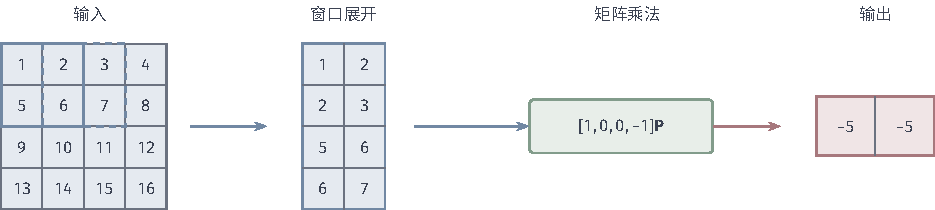
\includegraphics[width=158.358mm]{figures/01-mathematical-preliminaries-upper/03-graphs-and-signals/tikz/cnn-matrix-algorithm/figure.pdf}
  \caption{局部点积如何成为矩阵乘法。图中只取前两个相邻窗口，按核行、核列的顺序展平成$\bm P$的两列；核按相同顺序展平成一行。矩阵乘法同时得到这两个窗口的输出，完整计算包含九列。这里画的是代数上的窗口矩阵，是否实际复制全部数值由工程实现决定。}
  \label{fig:cnn-matrix-algorithm}
\end{figure*}
矩阵化之后还可以选择不同的矩阵乘法算法。下面的Strassen改变块乘法数量，它从属于矩阵乘法这条计算路线，与是否显式保存窗口是两个问题。

\paragraph{Strassen递归乘法}
\label{sec:cnn-strassen}

先设$\bm A,\bm B$为同阶的$n\times n$方阵，$n$为偶数，且$\bm C=\bm A\bm B$。
将三个矩阵各划成$2\times2$个块，每块都是$(n/2)\times(n/2)$方阵，普通算法给出
\begin{equation}
  \begin{aligned}
    \bm C_{1,1}&=\bm A_{1,1}\bm B_{1,1}+\bm A_{1,2}\bm B_{2,1},\\
    \bm C_{1,2}&=\bm A_{1,1}\bm B_{1,2}+\bm A_{1,2}\bm B_{2,2},\\
    \bm C_{2,1}&=\bm A_{2,1}\bm B_{1,1}+\bm A_{2,2}\bm B_{2,1},\\
    \bm C_{2,2}&=\bm A_{2,1}\bm B_{1,2}+\bm A_{2,2}\bm B_{2,2}\text{。}
  \end{aligned}
  \label{eq:cnn-classical-block-product}
\end{equation}
四个输出各含两次块乘法，共需八次。Strassen算法用七个组合块乘积替代这八次乘法，定义
\begin{equation}
  \begin{aligned}
    \bm M_1&=(\bm A_{1,1}+\bm A_{2,2})(\bm B_{1,1}+\bm B_{2,2}),\\
    \bm M_2&=(\bm A_{2,1}+\bm A_{2,2})\bm B_{1,1},\\
    \bm M_3&=\bm A_{1,1}(\bm B_{1,2}-\bm B_{2,2}),\\
    \bm M_4&=\bm A_{2,2}(\bm B_{2,1}-\bm B_{1,1}),\\
    \bm M_5&=(\bm A_{1,1}+\bm A_{1,2})\bm B_{2,2},\\
    \bm M_6&=(\bm A_{2,1}-\bm A_{1,1})(\bm B_{1,1}+\bm B_{1,2}),\\
    \bm M_7&=(\bm A_{1,2}-\bm A_{2,2})(\bm B_{2,1}+\bm B_{2,2})\text{。}
  \end{aligned}
  \label{eq:cnn-strassen-products}
\end{equation}
由这些结果恢复输出：
\begin{equation}
  \begin{aligned}
    \bm C_{1,1}&=\bm M_1+\bm M_4-\bm M_5+\bm M_7,\\
    \bm C_{1,2}&=\bm M_3+\bm M_5,\qquad
    \bm C_{2,1}=\bm M_2+\bm M_4,\\
    \bm C_{2,2}&=\bm M_1-\bm M_2+\bm M_3+\bm M_6\text{。}
  \end{aligned}
  \label{eq:cnn-strassen-recovery}
\end{equation}
这种组合靠的是多余项的抵消，而不是省略某个输入块。以左上输出为例，把四个中间量按左因子归并，有
\begin{equation}
  \begin{aligned}
    \bm M_1+\bm M_4-\bm M_5+\bm M_7
    ={}&\bm A_{1,1}(\bm B_{1,1}+\bm B_{2,2}-\bm B_{2,2})\\
       &+\bm A_{1,2}(-\bm B_{2,2}+\bm B_{2,1}+\bm B_{2,2})\\
       &+\bm A_{2,2}(\bm B_{1,1}+\bm B_{2,2}+\bm B_{2,1})\\
       &-\bm A_{2,2}(\bm B_{1,1}+\bm B_{2,1}+\bm B_{2,2})\\
    ={}&\bm A_{1,1}\bm B_{1,1}+\bm A_{1,2}\bm B_{2,1}\text{。}
  \end{aligned}
  \label{eq:cnn-strassen-cancellation}
\end{equation}
展开过程没有交换左右因子，因而对矩阵块同样成立。其余三个输出也可按式\eqref{eq:cnn-strassen-recovery}验证。核查例子取
\[
  \bm A=\begin{bmatrix}1&2\\3&4\end{bmatrix},\qquad
  \bm B=\begin{bmatrix}5&6\\7&8\end{bmatrix}\text{。}
\]
七个中间乘积依次为$65,35,-2,8,24,22,-30$，恢复后的结果是$\left[\begin{smallmatrix}19&22\\43&50\end{smallmatrix}\right]$，与普通乘法一致。

这一层递归将八次块乘法降为七次，块加减却从四次增为十八次，其中十次用于形成乘法输入，八次用于恢复输出。对$n\times n$方阵递归时，每个子问题的边长减半，加减的工作量仍与本层全部元素数成正比，因此$T(n)=7T(n/2)+O(n^2)$，得到$O(n^{\log_2 7})$。指数降低来自每层少一个乘法子问题，额外加减则是所支付的代价\scite{strassen1969}。

实现时通常只递归到合适阈值，底层仍调用高效GEMM；奇数尺寸需要拆分尾部或补齐，临时块应复用，某些加减可并入数据打包。卷积可在式\eqref{eq:signal-analysis-window-matrix-product}的矩阵乘法阶段接入该算法，但$c_{\mathrm{out}}\times q$与$q\times n_{\mathrm{win}}$常高度不对称，盲目补成方阵会浪费大量工作。递归、额外加减与写回可能抵消节省；相减还会改变舍入误差的传播。Strassen是可用的矩阵算法路线，不能由渐近指数直接推出它适合每次网格滤波。

\subsection{基于傅里叶变换的卷积计算}\label{sec:signal-analysis-fast-fft}\label{sec:cnn-fft}

矩阵路线把短点积集中起来交给更高效的乘法，但它本身的乘加量没有下降。
要真正减少乘法，需要换一组坐标，使原本要逐个乘积相加的运算变成逐点相乘。
上一节已经证明循环卷积在频率坐标下正是逐项相乘：核的DFT系数就是循环卷积算子的特征值。
整条路线的代价由此分成两部分：变换、逐点相乘、反变换。
若每个频率还要用定义逐项求和来算，这组三步比直接卷积更贵，
所以这条路线的成立还依赖一项独立的事实：DFT本身可以远快于定义式计算。

直接求$N$个DFT系数需要$O(N^2)$运算，再调用卷积定理并未自动提速。
\term{快速傅里叶变换}（fast Fourier transform, FFT）是一族快速计算DFT的算法，
不是另一种频率变换。它省下运算的方式是让不同频率的计算共用中间结果：
先把序列按偶数位置和奇数位置分成两半，两半各自的变换长度减半，
再把它们组合出全部频率的系数。基二Cooley--Tukey分解利用偶数长度的单位根结构复用子结果，
正是这一做法\scite{cooley1965fft}。
令$x_{\mathrm e}[r]=x[2r]$、$x_{\mathrm o}[r]=x[2r+1]$，
它们的$N/2$点DFT为$E[k],O[k]$。因为$\omega_N^2=\omega_{N/2}$，
\[
  \widehat x[k]
  =\sum_{r=0}^{N/2-1}x[2r]\omega_{N/2}^{kr}
   +\omega_N^k\sum_{r=0}^{N/2-1}x[2r+1]\omega_{N/2}^{kr}.
\]
而$\omega_N^{N/2}=-1$，子变换以$N/2$为周期，所以对$0\leq k<N/2$有蝶形关系
\begin{align}
  \widehat x[k]&=E[k]+\omega_N^kO[k],\notag\\
  \widehat x[k+N/2]&=E[k]-\omega_N^kO[k].
  \label{eq:signal-analysis-fft-butterfly}
\end{align}
\BookEquationAliases{\label{eq:cnn-fft-butterfly}}
同一对中间结果产生两个频率，没有舍弃后一半。
当$N=2^q$时，$T(N)=2T(N/2)+O(N)$，共$q$层、每层$O(N)$运算，
所以复杂度为$O(N\log N)$。
其他合数长度可按其他因子分解，质数长度也有相应算法；
补到二的幂只是某些实现的便利选择，不是FFT的普遍必要条件。

贯穿例补零到$N=4$，取$\bm x_4=(1,2,1,0)$、$\bm h_4=(1,-1,0,0)$。
$x_4$的偶分支$(1,1)$的二点DFT为$(2,0)$，奇分支$(2,0)$的为$(2,2)$。
用$\omega_4=-\mathrm i$合并得到
\[
  \widehat{\bm x}_4=(2+2,\ 0-2\mathrm i,\ 2-2,\ 0+2\mathrm i)
  =(4,-2\mathrm i,0,2\mathrm i).
\]
$h_4$的偶、奇分支DFT分别为$(1,1)$与$(-1,-1)$，同样得到
$\widehat{\bm h}_4=(0,1+\mathrm i,2,1-\mathrm i)$。
这一步显示如何复用两个二点变换，而不只是代入四点定义。
对$x_4$逆变换的四个分子依次为
\[
  4-2\mathrm i+2\mathrm i,\quad 4+2+2,\quad
  4+2\mathrm i-2\mathrm i,\quad 4-2-2,
\]
除以$4$后恢复$(1,2,1,0)$，同时核对了频率顺序、指数符号及归一化。
逐点乘积
$\widehat{\bm x}_4\odot\widehat{\bm h}_4=(0,2-2\mathrm i,0,2+2\mathrm i)$，
逆DFT给出$(1,1,-1,-1)$。若只用$N=3$，得到的是$(0,1,-1)$，
因为末项已经回绕；再精确的FFT也不能把这个循环输出当作原完整卷积。

\paragraph{长输入的分块计算}

对长输入作一次整体变换会占用较大工作区。FFT算法也可以逐块计算，以限制变换规模。\term{重叠相加}（overlap-add）将输入分块，每块补零后计算完整线性卷积，再将重叠的输出贡献相加；\term{重叠保留}（overlap-save）则让相邻输入块保留核长减一的重叠，只输出每块中没有循环污染的部分。一维核长$k\geq1$、变换长度$N\geq k$时，每块可保留$N-k+1$个新输出。例如将$(1,2,3,4)$拆为$(1,2)$与$(3,4)$，分别和$(1,-1)$作完整卷积，得到$(1,1,-2)$与$(3,1,-4)$。第二块原本从位置二开始，恢复后也要平移两位；重叠位置的$-2$与$3$相加，便得到整段输出$(1,1,1,1,-4)$，见图~\ref{fig:cnn-fft-blocks}。每块内部仍须补零至至少$2+2-1=3$，分块不能消除线性卷积的补零要求。

重叠保留选择另一种组织方式。取核长二、$N=4$，每个输入块保留前一块最后一个输入值，再接三个新值。首块为$(0,1,2,3)$，其循环卷积为$(-3,1,1,1)$；丢掉受回绕污染的第一项，保留$(1,1,1)$。下一块为$(3,4,0,0)$，保留结果$(1,-4,0)$，按目标长度截取前两项，仍恢复同一个完整输出。图~\ref{fig:cnn-fft-blocks}右侧将这一步与重叠相加并列。重叠相加在输出端相加，重叠保留在输入端重叠并丢弃污染位置，两者不能混用拼接规则。

\begin{figure*}[htb]
  \centering
  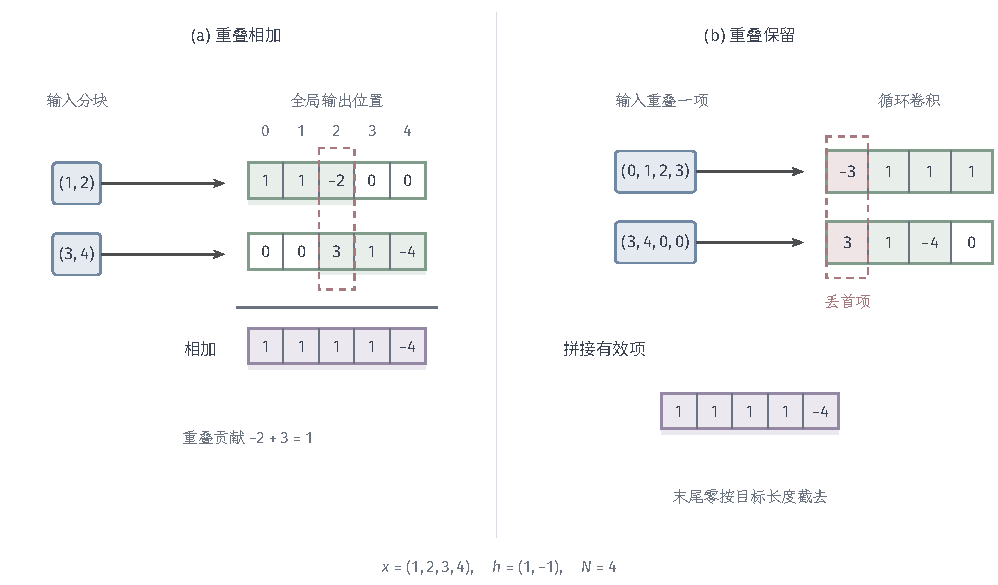
\includegraphics[width=168.998mm]{figures/01-mathematical-preliminaries-upper/03-graphs-and-signals/tikz/cnn-fft-blocks/figure.pdf}
  \caption{同一输入$(1,2,3,4)$与核$(1,-1)$的两种分块计算，均取$N=4$。
  左图把两个完整块卷积放回全局位置，红虚线框中的贡献$-2$与$3$相加为$1$。
  右图让相邻输入块重叠一项，丢弃红框中的循环污染首项，再拼接其余输出；
  末尾补零产生的多余输出按目标长度截去。两条计算链均恢复五项完整线性卷积，
  输出相加与污染项丢弃是不同的拼接规则。}
  \label{fig:cnn-fft-blocks}
\end{figure*}

块太小使变换和重叠开销增加，块太大增加内存及延迟。复数数组、变换代价与跨步后被丢弃的输出，都会影响分块是否减少总耗时。

\subsection{基于多项式插值的卷积计算}\label{sec:signal-analysis-fast-toom}\label{sec:cnn-toom-cook}

FFT用单位根这一组特殊选点换取快速变换，代价是对长度和复数运算有要求。
把卷积写成多项式乘法以后还可以看出，减少乘法的关键并不在于选点是否为根：
只要能在若干坐标处取到两个多项式的值，算出这些值两两相乘的结果，
再插值恢复系数，就同样完成了乘法。这条路线的优势是选点可以自由，
因而能针对小核、整数系数或短输出块作具体设计；代价是恢复过程需要另行求解。

Toom--Cook方法对多项式分块、求值、逐点相乘，再插值恢复系数。
先取输入$X(z)=x_0+x_1z$与核$K(z)=k_0+k_1z$。这两个次数至多为一的多项式可用$0,1,\infty$三个坐标相乘，其中$\infty$表示读取约定最高幂次位置的系数，
这里分别为$x_1$与$k_1$，允许为零。令$m_0=x_0k_0$、$m_\infty=x_1k_1$、$m_1=(x_0+x_1)(k_0+k_1)$，则
\begin{equation}
  (x_0+x_1z)(k_0+k_1z)
  =m_0+(m_1-m_0-m_\infty)z+m_\infty z^2\text{。}
  \label{eq:cnn-toom-example}
\end{equation}
中间系数本来是$x_0k_1+x_1k_0$，现在通过一次组合乘法减去两端乘积得到。四次数据与核之间的乘法降为三次；这一最小例子也称Karatsuba乘法。例如$\bm x=(1,2)$、$\bm k=(1,-1)$时，三个乘积为$1,0,-2$，恢复得到系数$(1,1,-2)$。


这一组合乘法也可用于更多系数。对次数至多为二的$X$与次数至多为一的$H$，乘积次数至多为$3$，
可使用$0,1,-1,\infty$四个坐标；其中“无穷点”表示读取约定最高幂次位置的系数，
不是把无穷大传给数值程序\scite{math-knuth1997seminumerical}。
记
\begin{align}
  r_0&=X(0)H(0),&r_+&=X(1)H(1),\notag\\
  r_-&=X(-1)H(-1),&r_\infty&=x_2h_1.\label{eq:cnn-toom-three-two-evaluation}
\end{align}
设$P(z)=c_0+c_1z+c_2z^2+c_3z^3$，
则$r_+=c_0+c_1+c_2+c_3$，$r_-=c_0-c_1+c_2-c_3$，
和、差分别解出偶次与奇次部分：
\begin{align}
  c_0&=r_0,\qquad c_3=r_\infty,\notag\\
  c_1&=\frac{r_+-r_-}{2}-c_3,\notag\\
  c_2&=\frac{r_++r_-}{2}-c_0.
  \label{eq:signal-analysis-toom-reconstruction}
\end{align}
\BookEquationAliases{\label{eq:cnn-toom-three-two-recovery}}
这是前述插值思想在包含最高次坐标时的具体形式；分母$2$要求系数域中$2$可逆。

贯穿例的四个值为$(r_0,r_+,r_-,r_\infty)=(1,0,0,-1)$，
恢复为$(c_0,c_1,c_2,c_3)=(1,1,-1,-1)$。
直接展开需$3\times2=6$次输入系数与核系数相乘，此方案只需四次点值乘法，
却增加了求值、插值及常数乘除。长多项式可递归分块获得渐近改进，
短核则未必值得；缓存、数据变换和访存也要计入。
点值乘法之所以成立，是因为$P(a)=X(a)H(a)$，不是因为任意坐标变换都把乘法变为逐点乘法。

\paragraph{三段分块与递归}

三段分块进一步展示插值过程。对两个次数至多为二的多项式，在$0,1,-1,2,\infty$求值并相乘，记结果为$r_0,r_1,r_{-1},r_2,r_\infty$。这里使用实数或复数系数，除以$2$和$3$都有定义；其他系数域须检查二者是否可逆。乘积次数至多为四，正好需要五个条件：$c_0,c_4$由两端直接给出；$r_1+r_{-1}$分离偶数次项，$r_1-r_{-1}$给出$c_1+c_3$；再用$r_2$区分这两个奇数次系数。乘积系数$c_0,\ldots,c_4$可按下式恢复：
\begin{equation}
  \begin{aligned}
    c_0&=r_0,\qquad c_4=r_\infty,\\
    c_2&=(r_1+r_{-1})/2-c_0-c_4,\\
    v&=(r_1-r_{-1})/2,\\
    u&=(r_2-c_0-4c_2-16c_4)/2,\\
    c_3&=(u-v)/3,\qquad c_1=v-c_3\text{。}
  \end{aligned}
  \label{eq:cnn-toom-three}
\end{equation}
这里$u,v$只是插值中间量。五次求值后的乘法替代九次原始系数乘法，但新增了求值加减、常数乘除和插值。例如$\bm x=(1,2,3)$、$\bm k=(1,-1,2)$的五个点值乘积是$1,12,8,119,6$；式\eqref{eq:cnn-toom-three}先给出$c_2=3,v=2,u=5$，再得到$c_3=1,c_1=1$，完整输出为$(1,1,3,1,6)$。

长序列可以每$\ell$项分为一段，写成$X(z)=X_0(z)+z^\ell X_1(z)+z^{2\ell}X_2(z)$，核也同样分段。把$z^\ell$暂看成外层变量，刚才的五次乘法就变为五个短多项式乘法；每个段内乘积再递归计算。插值后将第$j$个段内结果平移$j\ell$位，并把重叠系数相加。对两条长度相近的序列，三等分递归满足$T(n)=5T(n/3)+O(n)$，理想成本为$O(n^{\log_3 5})$；它不能直接作为长输入与短滤波核的复杂度，因为两者形状并不相近。

实现需选择分块长度和求值点，保存或流式产生求值结果，并把恢复的系数按原位置累加。求值点过大或插值中出现相近量相减，可能放大浮点误差；低精度下尤其要检查变换后的动态范围。数学卷积与互相关可通过共轭反转核及相应的输出选段建立对应，但局部滤波通常只需一小段输出，计算完整多项式乘积可能浪费工作。Toom--Cook解释了“用变换交换乘法与加法”的一般思路，接下来的Winograd则直接面向小块滤波输出。

\subsection{基于余数分解的卷积计算}\label{sec:signal-analysis-fast-winograd}\label{sec:cnn-winograd}

Toom--Cook按次数界选择一组点，恢复的是整条乘积的全部系数。
实际滤波有时只需要少数几个相邻输出，算出完整乘积会浪费大半工作，
而且不同输出块的恢复公式还得分别推导。
上一小节建立的多项式工具提供了另一条出路：把多项式换成关于几个低次模的余数，
在这些余数上相乘，再用中国剩余定理拼回去。
余数比点值自由，因为模不限于一次多项式；
若模是一次多项式，余数就是一个数，这一路线便退化为点值插值。
当任务只要一小块输出时，可以选择只恢复所需系数的那组模，
从而在减少乘法的同时避免算不需要的部分。

Winograd类算法据此构造较少乘法的乘积或滤波计算，特定输出块还需相应的恢复映射
\scite{math-winograd1980arithmetic}。
回到贯穿例，令$X(z)=1+2z+z^2$、$H(z)=1-z$，
完整乘积仍为$P(z)=X(z)H(z)=1+z-z^2-z^3$。先取
$M(z)=z^4-1=(z-1)(z+1)(z^2+1)$。
三个实系数因子两两互素、总次数为$4$，分别有
\[
  P(1)=0,\quad P(-1)=0,\qquad
  X\bmod(z^2+1)=2z,\quad H\bmod(z^2+1)=1-z.
\]
在第三个模下$z^2=-1$，所以$XH\equiv2+2z$。
设恢复的$R$次数小于$4$，前两份零余数使
$R(z)=(z^2-1)(az+b)$。再模$z^2+1$得到$R\equiv-2az-2b$，
与$2+2z$比较便有$a=b=-1$，从而$R=1+z-z^2-z^3$。
原乘积次数已经小于$4$，因此这正是完整乘积；若次数更高，就只能得到模代表元。
本次映射从长度$3$和$2$的输入恢复四项完整卷积，不能直接称作任意输出块的最小算法。

回到长度三与长度二的乘积，沿用式\eqref{eq:cnn-toom-three-two-evaluation}，选取$z,z-1,z+1$，其乘积为$M(z)=z^3-z$。用$S$记式~\eqref{eq:signal-analysis-toom-reconstruction}所恢复的乘积。由于$S$次数至多为三、最高次项系数是$r_\infty$，可写成
\begin{equation}
  S(z)=r_\infty M(z)+R(z),\qquad \deg R<3\text{。}
  \label{eq:cnn-winograd-polynomial-remainder}
\end{equation}
在$0,1,-1$处，$M$都为零，故$R$保留$S$在这三点的值$r_0,r_+,r_-$。下面三个二次多项式各自在一个点等于一、在另外两点等于零：
\[
  L_0(z)=1-z^2,\quad
  L_+(z)=(z^2+z)/2,\quad
  L_-(z)=(z^2-z)/2\text{。}
\]
因而余数的具体重构式是
\begin{equation}
  R(z)=r_0L_0(z)+r_+L_+(z)+r_-L_-(z)\text{。}
  \label{eq:cnn-winograd-remainder-reconstruction}
\end{equation}
代入并展开$r_\infty(z^3-z)+R(z)$，就得到式\eqref{eq:cnn-toom-three-two-recovery}的四项系数。该例中一次基多项式的余数就是点值，所以余数重构与Toom--Cook插值给出同一个计算过程；选择更一般的基多项式时，余数也可能是低次多项式，而非一个数值。

\paragraph{从完整卷积转为小块滤波}

固定长度三的实核$\bm g=(g_0,g_1,g_2)^\top$，将它与长度二的实向量$\bm b$作完整数学卷积，可写为$\bm s=\bm H_{\bm g}\bm b$，其中
\begin{equation}
  \bm H_{\bm g}=\begin{bmatrix}
    g_0&0\\g_1&g_0\\g_2&g_1\\0&g_2
  \end{bmatrix},\qquad
  \bm H_{\bm g}^\top\bm d=
  \begin{bmatrix}
    d_0g_0+d_1g_1+d_2g_2\\
    d_1g_0+d_2g_1+d_3g_2
  \end{bmatrix}\text{。}
  \label{eq:cnn-winograd-filter-transposition}
\end{equation}
右侧正是长度四实输入$\bm d$经过该实核产生的两个互相关输出。把前面完整卷积的线性计算图转置，就可将“两个输入、四个完整输出”变为“四个输入、两个有效输出”，核心乘法仍为四次。

更具体地，若完整卷积算法写为$\bm s=\bm R[(\bm E\bm g)\odot(\bm Q\bm b)]$，其中$\bm E,\bm Q$负责求值、$\bm R$负责恢复，则固定核后，整个映射是$\bm R\operatorname{Diag}(\bm E\bm g)\bm Q$。转置后得到
\[
  \bm H_{\bm g}^\top\bm d
    =\bm Q^\top[(\bm E\bm g)\odot(\bm R^\top\bm d)]\text{。}
\]
这里$\operatorname{Diag}$把向量放到对角线上；转置只反转线性变换的顺序，逐项乘法仍使用相同的四个核组合。将固定系数$1/2$在数据变换与核变换之间重新分配，就得到下面常用的公式。整个构造依赖转置的乘积规则，不要求输入或输出变换可逆。

以下记$F(p,r)$为用$r$项核计算$p$个相邻valid互相关输出的构造，所需输入长度为$p+r-1$。

\begin{example}[可复核的Winograd \(F(2,3)\)输出块]
  \label{ex:signal-analysis-winograd-f23}
  固定一维valid互相关，输入$\bm d=(d_0,d_1,d_2,d_3)^\top$，
  核$\bm g=(g_0,g_1,g_2)^\top$，所需输出只有
  \begin{align*}
    y_0&=d_0g_0+d_1g_1+d_2g_2,\\
    y_1&=d_1g_0+d_2g_1+d_3g_2.
  \end{align*}
  $F(2,3)$使用关于$z,z-1,z+1$的余数与最高次系数坐标。
  核侧是$0,1,-1$处点值及最高次系数的缩放；
  输入侧则针对只恢复两项输出另作线性组合。一组符合本章方向约定的变换为
  \begin{equation}
    \bm y=\bm A^\top\bigl[(\bm G\bm g)\odot(\bm B^\top\bm d)\bigr],
    \label{eq:signal-analysis-winograd-f23}
  \end{equation}
\BookEquationAliases{\label{eq:cnn-winograd-matrix-a}
\label{eq:cnn-winograd-matrices-bg}
\label{eq:cnn-winograd-recovery-principle}
\label{eq:cnn-winograd-one-dimensional}
\label{eq:cnn-winograd-vector-transform}}
  其中
  \begin{align*}
    \bm B^\top&=\begin{bmatrix}
      1&0&-1&0\\0&1&1&0\\0&-1&1&0\\0&1&0&-1
    \end{bmatrix},\\
    \bm G&=\begin{bmatrix}
      1&0&0\\1/2&1/2&1/2\\1/2&-1/2&1/2\\0&0&1
    \end{bmatrix},\\
    \bm A^\top&=\begin{bmatrix}1&1&1&0\\0&1&-1&-1\end{bmatrix}.
  \end{align*}
  形状分别为$\mathbb R^4\to\mathbb R^4$、$\mathbb R^3\to\mathbb R^4$，
  逐点相乘后由$\mathbb R^4\to\mathbb R^2$恢复指定输出。
  为直接核对恒等式，记
  \begin{align*}
    m_1&=(d_0-d_2)g_0,\\
    m_2&=\tfrac12(d_1+d_2)(g_0+g_1+g_2),\\
    m_3&=\tfrac12(-d_1+d_2)(g_0-g_1+g_2),\\
    m_4&=(d_1-d_3)g_2.
  \end{align*}
  则$m_2+m_3=d_2g_0+d_1g_1+d_2g_2$，
  $m_2-m_3=d_1g_0+d_2g_1+d_1g_2$，
  所以$m_1+m_2+m_3=y_0$、$m_2-m_3-m_4=y_1$。

图~\ref{fig:cnn-winograd-example}取$\bm d=(1,2,3,4)$、$\bm g=(1,2,3)$，得到$\bm m=(-2,15,1,-6)$，再恢复$(14,20)$；直接计算也给出$1+4+9=14$和$2+6+12=20$。输入变换需要四次加减，核变换可用三次加减与两次乘以$1/2$，输出恢复需要四次加减。含$1/2$的核变换可在核系数不变时复用，不应把全部变换开销计为零。


\end{example}

\begin{figure*}[htb]
  \centering
  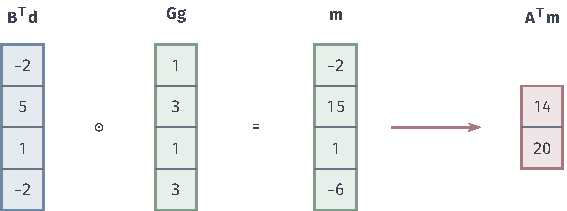
\includegraphics[width=95.934mm]{figures/01-mathematical-preliminaries-upper/03-graphs-and-signals/tikz/cnn-winograd-example/figure.pdf}
  \caption{一维$F(2,3)$的完整数值路径。输入$\bm d=(1,2,3,4)^\top$与核$\bm g=(1,2,3)^\top$分别变为四个组合值，按位置相乘得到$\bm m=(-2,15,1,-6)^\top$，再用输出变换恢复两个互相关结果。四次核心乘法替代直接算法的六次乘法，加减与固定系数变换仍有成本。}
  \label{fig:cnn-winograd-example}
\end{figure*}

\paragraph{沿两个轴组合变换}

复用上述三个矩阵，把一维变换沿两个轴组合，$3\times3$核$\bm K$与$4\times4$输入块$\bm D$产生$2\times2$输出：
\begin{equation}
  \begin{aligned}
    \bm U&=\bm G\bm K\bm G^\top,\qquad
    \bm V=\bm B^\top\bm D\bm B,\\
    \bm Y&=\bm A^\top(\bm U\odot\bm V)\bm A\text{。}
  \end{aligned}
  \label{eq:cnn-winograd-transform}
\end{equation}
左乘组合第一索引轴上的值，右乘组合第二索引轴上的值；因此$\bm U,\bm V$均为$4\times4$，逐元素乘积有十六项，输出恢复将其变为$2\times2$。这不是对每个输出独立使用一维技巧，而是两轴都先形成组合，再让十六个乘积服务于全部四个输出。直接计算的$4\times9=36$次核心乘法降为$16$次\scite{lavin2016fast}。

这些矩阵对应步长一、核读取间隔为一的$3\times3$核；改变读取规则时必须重新构造变换。核侧和输入侧的十六项变换值也要占用工作区，减少核心乘法并未免去变换成本。

\subsection{基于核分离的卷积计算}\label{sec:signal-analysis-fast-separable}
\label{sec:cnn-separable-implementation}

前面的路线从两个方面改变计算：矩阵化重新组织点积，并不减少普通乘加次数；
FFT、Toom--Cook与Winograd则在各自指定的输出范围和构造条件下，
利用变换减少核心乘法，同时付出变换与恢复的代价。
还有一类加速利用的是核自身的代数结构：若二维核$k_{a,b}$恰好可以写成
一个列向量$u_a$与一个行向量$v_b$的乘积$u_av_b$，那么二维加权求和就可以拆成两个方向的
一维加权求和，乘法量从两轴长度之积降到两轴长度之和。
核是否具有这种结构由任务决定，不是算法能够选择的；
它成立时可以直接沿两轴先后滤波，不必先做频域变换；
但边界补值仍须与原二维滤波一致。实际节省多少，要比较两次一维滤波的输出范围、
中间数组以及核的长度，不能仅凭可分离就断言它总比其他路线更快。

若单通道核可写成$k_{a,b}=u_a v_b$，即$\bm K=\bm u\bm v^\top$，二维滤波就可分解为一个方向的长度$k_h$滤波和另一个方向的长度$k_w$滤波。这一分解直接来自求和顺序：
\begin{equation}
  \begin{aligned}
    t_{i,j}&=\sum_{b=0}^{k_w-1}v_bx_{i,j+b},\\
    y_{i,j}&=\sum_{a=0}^{k_h-1}u_at_{i+a,j}
      =\sum_{a=0}^{k_h-1}\sum_{b=0}^{k_w-1}
          u_av_bx_{i+a,j+b}\text{。}
  \end{aligned}
  \label{eq:cnn-spatial-separable-derivation}
\end{equation}
水平结果$t_{i,j}$可以被多个垂直窗口复用，因此不必为每个二维窗口重新计算整组水平点积。窗口逐格移动、核读取相邻索引且逐轴边界与裁剪一致时，在足够大的网格上，主要成本由每个输出附近的$k_hk_w$项降为约$k_h+k_w$项，代价是保存或流式处理一维中间结果。

取$\bm u=\bm v=(1,2,1)^\top$，则$\bm K=\left[\begin{smallmatrix}1&2&1\\2&4&2\\1&2&1\end{smallmatrix}\right]$。对式~\eqref{eq:signal-analysis-matrix-filter-example}中的$4\times4$输入，水平滤波先得到$4\times2$的中间矩阵，再垂直滤波得到$2\times2$输出，图~\ref{fig:cnn-spatial-separable}列出全部数值。左上输出为$8+2\times24+40=96$，与直接二维求和一致。

这个小例子也提醒我们区分局部估算与完整成本。设输入大小为$h\times w$且$h\geq k_h$、$w\geq k_w$，不填充且窗口逐格移动时，输出大小为$h'=h-k_h+1$、$w'=w-k_w+1$，中间矩阵尺寸是$h\times w'$，所以两阶段共需$hw'k_w+h'w'k_h$次核心乘法，并不严格等于$h'w'(k_h+k_w)$。本例需要$4\times2\times3+2\times2\times3=36$次，与直接计算的$2\times2\times9=36$次相同；对$100\times100$输入，同一核的两阶段成本为$58212$次，直接计算则为$86436$次。图像相对核越大，中间区域的额外边界开销越容易摊薄。
\begin{figure*}[htb]
  \centering
  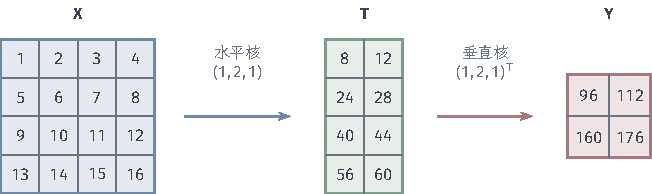
\includegraphics[width=110.335mm]{figures/01-mathematical-preliminaries-upper/03-graphs-and-signals/tikz/cnn-spatial-separable/figure.pdf}
  \caption{秩一空间核的两阶段计算。水平核与垂直核均为$(1,2,1)$，组成$3\times3$核$\bm u\bm v^\top$。在步长一、无填充条件下，原$4\times4$输入先变为$4\times2$中间结果，再变为$2\times2$输出。该小例子的两阶段核心乘法量仍为三十六次，图示验证的是结果等价，而非每种输入尺寸都能节省计算。}
  \label{fig:cnn-spatial-separable}
\end{figure*}


一般核未必秩一。对核作奇异值分解，将第$r$个奇异值吸收到一个向量中，得到核$\bm K_\rho=\sum_{r=1}^{\rho}\bm u_r\bm v_r^\top$，其中$\rho$为保留的非零奇异值个数。保留全部非零奇异值时，$\bm K_\rho=\bm K$；计算$\rho$组一维滤波并相加，即可恢复原二维核的输出。在大网格上的每位置主要成本约为$\rho(k_h+k_w)$，只有这比$k_hk_w$足够小，才可能抵消分解与中间读写。只保留较少的奇异值通常会改变输出，属于近似算法，应检查输出误差。这里分解的是单个空间核的两个轴，没有改变输入通道和输出通道之间的连接关系。

\begin{table*}[htb]
  \centering
  \begin{tabularx}{\linewidth}{@{}lXX@{}}
    \toprule
    计算路线 & 计算过程的改变 & 适用条件与代价\\
    \midrule
    直接计算 & 枚举全部局部乘积并累积 & 适用各种采样设置，乘加量为窗口数、窗口长度与输出通道数的乘积\\
    矩阵化计算 & 将点积集中为矩阵乘法 & 普通GEMM保持乘加量；Strassen可减少块乘法，但增加加减与误差敏感性\\
    Toom--Cook & 求值、逐点乘法、插值 & 面向多项式乘积，可能计算不需要的输出系数\\
    Winograd & 固定变换恢复小块滤波输出 & 小核、小步长设置；变换成本及数值条件需核对\\
    FFT & 频域乘法后反变换 & 线性卷积须补零，变换与复数运算有成本\\
    空间可分离核 & 低秩分解为一维滤波 & 无损计算要求相应低秩结构；截断分解会改变输出\\
    \bottomrule
  \end{tabularx}
  \caption{按计算过程比较卷积算法。矩阵化本身不减少普通乘加量，但提供了选择矩阵乘法算法的入口。前五条路线在精确算术下、满足各自的边界与输出条件时恢复指定的卷积或互相关；空间可分离路线还要求核具有相应结构。表中不把显式展开、隐式取数等存储选择作为新的代数算法。}
  \label{tab:cnn-algorithms}\label{tab:signal-analysis-convolution-algorithms}
\end{table*}

图~\ref{fig:cnn-transform-algorithms}把三类变换放在同一条输入、乘法和恢复路径上；它们的区别在于坐标的选择与要恢复的输出。
\begin{figure*}[tb]
  \centering
  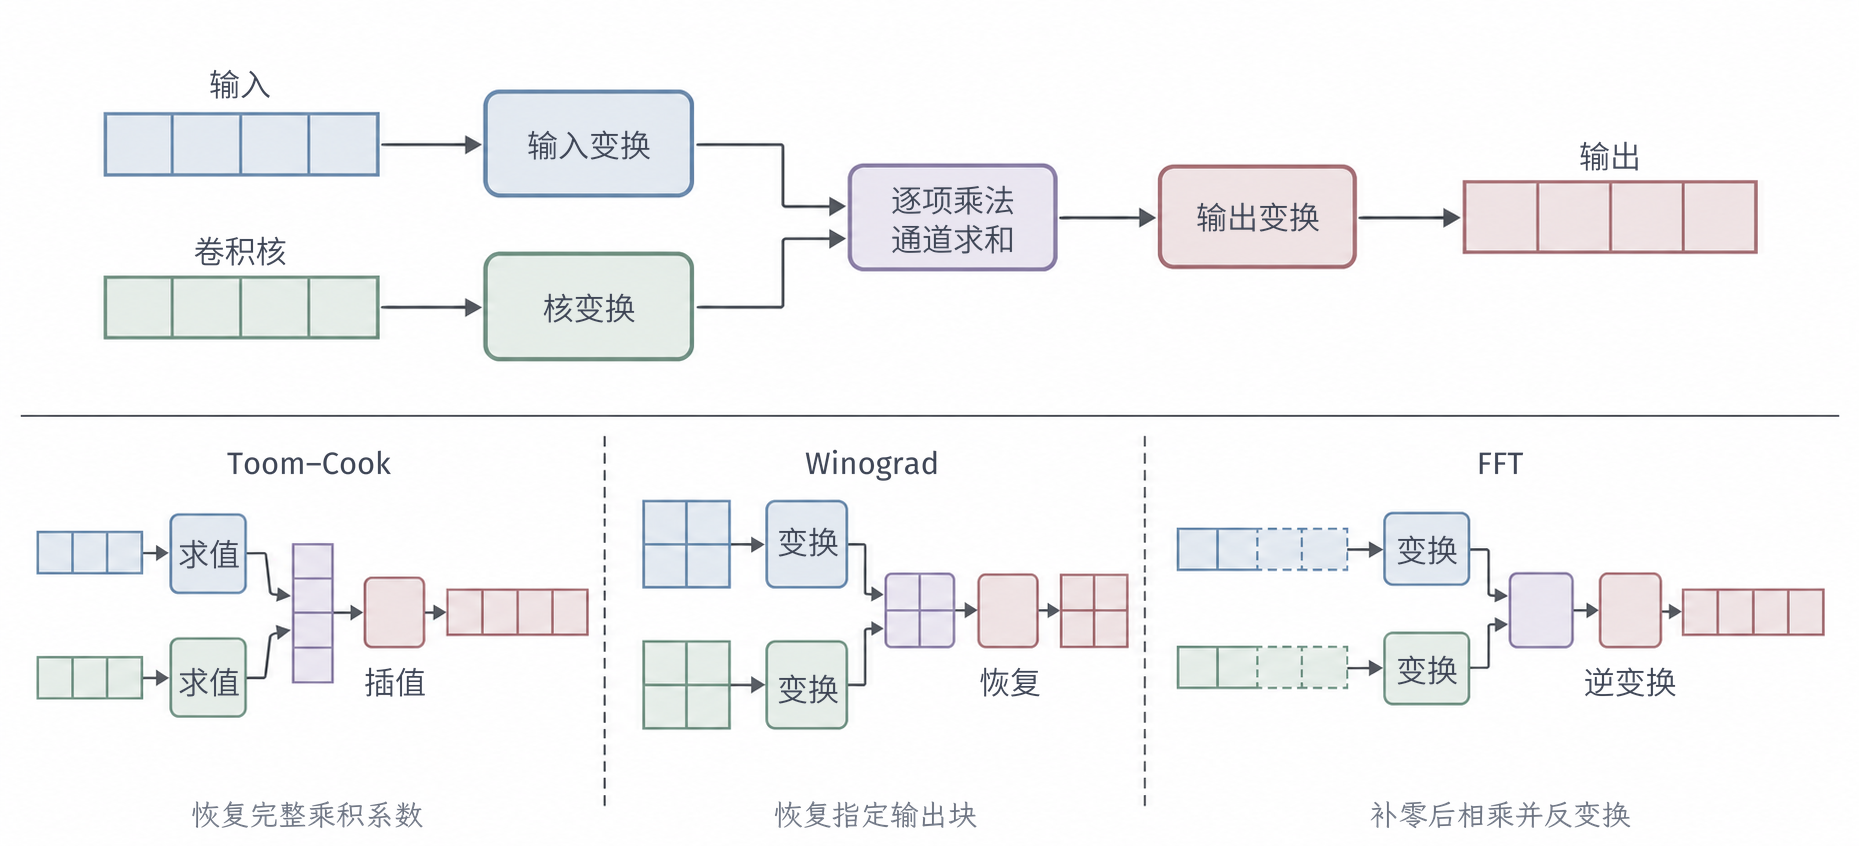
\includegraphics[width=169mm]{figures/01-mathematical-preliminaries-upper/03-graphs-and-signals/generated/cnn-transform-algorithms/figure.png}
  \caption{变换类卷积的共同流程与不同目标。Toom--Cook通过多项式求值及插值恢复完整乘积系数；Winograd通过固定小矩阵恢复所需输出块；FFT在补零后的频域相乘并反变换。输入和核可以分别变换，变换结果按输入通道相乘并求和；能复用多少次，决定变换开销能否被摊薄。格子只示意数组，不表示具体尺寸或数值。}
  \label{fig:cnn-transform-algorithms}
\end{figure*}

矩阵路线把窗口点积汇集为一个乘法；三类变换路线利用乘法兼容的表示，结构却不同。
FFT在$z^N-1$的全部复单位根处求值，并利用根的规则结构快速变换；
Toom--Cook允许一般选点及递归分块；Winograd类构造用互素余数并常针对指定小块输出。
一次因子的CRT与点值插值重合，高次因子保留的却是一个低次多项式，不能称为单个点值。

长度相近的两个$n$项序列直接卷积需要$O(n^2)$次乘加，
FFT路线在合适长度上需$O(N\log N)$变换运算及$N$次频域乘法。
乘法数和渐近量级并非完整运行时间：加减、复数算术、常数运算、缓存复用与目标硬件
都会改变实际排序。归一化DFT是酉变换、条件良好，但多层蝶形仍会累积舍入误差；
Toom--Cook和Winograd的变换矩阵可能有较大尺度差异，相近量相减也会放大相对误差。

整数或有限域算法还要检查系数域条件。一个有限域（finite field）的例子是
模素数$p$的数系：只保留$0,\ldots,p-1$，加乘后取模，非零元素都有乘法逆元。
例如模$5$时$2\cdot3=1$，所以除以$2$就是乘以$3$。
数论变换（number-theoretic transform, NTT）在这类数系中按DFT的形式求值；
它需要所需阶数的单位根，逆变换中的$N$也须可逆。
若$p$整除$N$，$N$在该数系中就是零，不能作为除数；
前面Toom--Cook的除以$2$、$3$也有同样的系数域限制。

若目标是恢复整数系数，还要从有限域运算返回整数余数重构。
此处的模数是整数，与前面的模多项式不同。设总整数模数为$Q$
（使用多个两两互素模数时取它们的乘积），选取区间$(-Q/2,Q/2]$内的余数代表。
已知每个真实系数绝对值不超过$B$时，$Q>2B$保证该代表唯一等于真实系数：
两个候选系数之差绝对值至多$2B$，不可能是非零的$Q$倍数。
第$n$个卷积系数的绝对值可由$\sum_{i+j=n}|x_i h_j|$控制，
再对输出位置取统一上界即可选取$B$。
避免浮点误差并不等于避免模混淆或整数溢出。
没有脱离规模、数据类型和误差目标的普遍最优算法。

选择计算路线以后，还要核对它是否输出了所要求的映射。FFT计算完整线性卷积需要
足够补零；Toom--Cook恢复所设多项式乘积；互相关需要匹配核方向；Winograd恢复
构造时指定的小块输出。步长、核读取间隔或边界改变后，相应变换也要重新验证。
快速算法改变的是计算组织，输入与输出的含义仍由原问题确定。

\section{信号的采样与恢复}
\label{sec:signal-analysis-sampling}

前面各节都假定数据已经是数组，关心的是怎样表示和计算它。
但设备实际存下来的正是数组：传感器按固定间隔读出数值，
连续记录被压缩成一串有限精度的样本。若日后需要重建样本之间的取值、或改变采样间隔，
就要问清楚这一步转换丢失了什么。前面已经看到，DFT用同样多的频率坐标替换数组，
保留全部坐标便能精确还原每一项；这个结论容易被误读成“采样本身也没有损失”。
两者的对象不同：坐标换法可逆说的是数组与它的频率系数一一对应，
而原始连续信号在样本之间的取值从未进入数组，逆变换自然也无法凭数组把它们恢复出来。

要把这一步说清楚，需要先找一个具体的失败例子，看两条明显不同的连续信号怎样产出同一串样本。
有反例以后，再问需要补充什么条件才能排除它，这个条件就是后文的带限假设。
限制频率能保证恢复，但设备往往在采样前就已经先把高频压低，
这又改变了需要恢复的对象，于是还要单独讨论这一步预滤波做了什么。

\subsection{采样后的频率混叠}
\label{sec:signal-sampling-ambiguity}

固定时间原点及采样间隔$T_s>0$，对具有确定点值的连续时间信号$f$读取
$x[n]=f(nT_s)$，采样频率为$\nu_s=1/T_s$。
若不约束候选信号，采样通常不是单射。
例如$T_s=1$时，$f_1(t)=\cos(0.8\pi t)$与$f_2(t)=\cos(1.2\pi t)$频率不同，
却满足
\[
  f_2(n)=\cos(2\pi n-0.8\pi n)=\cos(0.8\pi n)=f_1(n),
  \qquad n\in\mathbb Z.
\]
这是\term{混叠}（aliasing）：不同连续振荡在样本上无法区分。
图~\ref{fig:signal-aliasing-curves}中的两条曲线在样本之间起伏不同，
但每个整数位置都穿过同一点。

同样的重合也可以用带量纲的采样率写出。设采样间隔$T_s=0.5$秒，
即采样频率$\nu_s=2$赫兹，那么$1$赫兹的余弦$\cos(2\pi t)$与$3$赫兹的余弦
$\cos(6\pi t)$在$t=0.5n$处同时给出
\[
  \cos(2\pi\cdot0.5n)=\cos(\pi n),\qquad
  \cos(6\pi\cdot0.5n)=\cos(3\pi n)=\cos(\pi n).
\]
两者样本完全相同，恢复时无法区分。这两个频率之和为$4$赫兹，恰为采样频率的两倍；
一般地，频率$f$与$\nu_s-f$在采样后不可区分，
偏离更远的频率则反复折回，落在$0$到$\nu_s/2$之间。
这个区间就是采样率能够分辨的频率范围，其右端点$\nu_s/2$称为Nyquist频率。
若信号的频率超过它，样本记录下来的只是折回后的低频振荡，原始快慢已经无法从样本判断。
\begin{figure}[htbp]
  \centering
  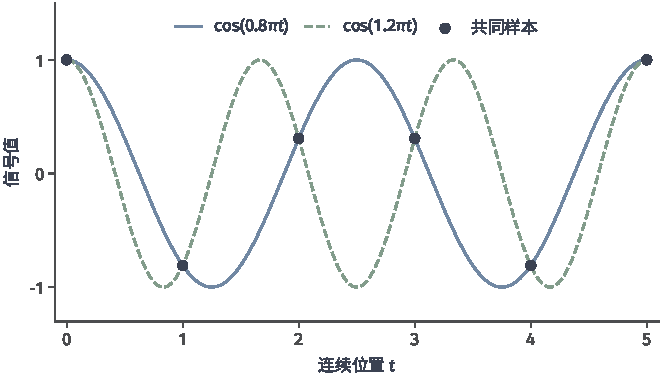
\includegraphics[width=112.0mm]{figures/01-mathematical-preliminaries-upper/03-graphs-and-signals/matplotlib/signal-aliasing-curves/figure.pdf}
  \caption{教学构造$f_1(t)=\cos(0.8\pi t)$与$f_2(t)=\cos(1.2\pi t)$。
  蓝色实线和绿色虚线在整数时刻具有共同样本，深灰圆点标出这些观测。
  图只展示$[0,5]$，样本相同对所有整数成立；两条纯余弦是功率信号，
  不属于后文定理中的整轴平方可积信号类。}
  \label{fig:signal-aliasing-curves}
\end{figure}

任何确定性插值器对相同输入样本只能返回同一输出，因此不可能同时正确恢复这两条曲线。
学习模型可以凭训练分布猜测更常见的细节，但这种能力来自额外先验，
不是采样映射自己变成可逆。这里的余弦有有限平均功率而整轴能量无穷，
只用于展示歧义；后文将换到$L^2$带限空间，不能把此例当作那个空间中的反例。
对一般$L^2$等价类，点值采样本身还未定义，下一小节会先补齐代表元条件。

离散信号也可以丢弃位置。对正整数$M$保留每$M$项中的一项，
$y[n]=x[Mn]$，称为$M$倍\term{下采样}（downsampling）。
其DTFT满足
\begin{equation}
  Y(e^{\mathrm i\omega})=\frac1M\sum_{\ell=0}^{M-1}
  X\left(e^{\mathrm i(\omega+2\pi\ell)/M}\right).
  \label{eq:signal-analysis-downsampling-spectrum}
\end{equation}
对$x\in\ell_1$，按定义展开右侧并交换有限和与绝对收敛级数，
\begin{align*}
  \frac1M\sum_{\ell=0}^{M-1}X\left(e^{\mathrm i(\omega+2\pi\ell)/M}\right)
  &=\sum_{r\in\mathbb Z}x[r]e^{-\mathrm ir\omega/M}
    \left(\frac1M\sum_{\ell=0}^{M-1}e^{-2\pi\mathrm i\ell r/M}\right)\\
  &=\sum_{n\in\mathbb Z}x[Mn]e^{-\mathrm i\omega n}.
\end{align*}
括号内的单位根和只在$M\mid r$时为$1$，否则为$0$，故留下的恰为输出DTFT。
对$x\in\ell_2$，下采样满足$\sum_n|x[Mn]|^2\leq\sum_r|x[r]|^2$，
频域右侧的有限分支映射在$L^2$中也有界；
先对有限截断证明再取$L^2$极限，便得到同一公式的等价类解释。

输入模式$e^{\mathrm i\omega_0n}$变为$e^{\mathrm iM\omega_0n}$，
输入频率映到$M\omega_0\bmod2\pi$。
原频谱沿输出频率轴扩展$M$倍，超出主值区间的部分回绕，与其他分量相加。
所以“样本点变少”不只是频率曲线画得稀疏，而可能直接合并原来不同的频率。
连续采样的频谱复制也有类似现象，但必须在可读取点值的信号类上推导。

\subsection{带限条件下的信号恢复}
\label{sec:signal-bandlimited-recovery}

前面的歧义来自两条不同频率的曲线具有相同样本。这里通过限制候选曲线
允许包含的频率来排除这种歧义。具体采用带限条件：在某个频率区间以外，频谱几乎处处为零。
\begin{definition}[平方可积带限信号]
  \label{def:signal-analysis-bandlimited-space}
  设$\Omega_{\max}>0$、$f\in L^2(\mathbb R)$，其Plancherel意义的傅里叶变换为$F$。
  若$F(\Omega)=0$对几乎处处的$|\Omega|>\Omega_{\max}$成立，
  称$f$带限于$\Omega_{\max}$。
  所有这类函数组成\term{Paley--Wiener带限空间}。
\end{definition}
只观察一个有限时间窗口，不能推出窗口外为零，更不能推出高频为零。
带限才是下面用来排除混叠的信号类条件。

带限还使点值有规范含义。由$F\in L^2$及频谱支撑长度有限，
Cauchy--Schwarz不等式给出
\[
  \|F\|_1\leq\sqrt{2\Omega_{\max}}\,\|F\|_2<\infty.
\]
因此
\[
  f_{\mathrm c}(t)=\frac1{2\pi}\int_{-\Omega_{\max}}^{\Omega_{\max}}
  F(\Omega)e^{\mathrm i\Omega t}\,\mathrm d\Omega
\]
是$f$的连续代表元。若$t_j\to t$，被积函数逐点趋于
$F(\Omega)e^{\mathrm i\Omega t}$，且绝对值均由可积函数$|F|$支配；
支配收敛定理使积分值趋于$f_{\mathrm c}(t)$，从而得到连续性。
两个连续代表元若几乎处处相等，就处处相等，所以这种选择唯一。
以下仍记它为$f$，样本$f(nT_s)$都针对这个代表元，不针对随意改过点值的版本。

记采样角频率$\Omega_s=2\pi/T_s$，基带
$I_s=[-\pi/T_s,\pi/T_s]$。这里\term{基带}（baseband）指选定的一段基本频率区间。
将频谱副本按间隔$\Omega_s$相加，
\[
  P_F(\Omega)=\frac1{T_s}\sum_{k\in\mathbb Z}F(\Omega-k\Omega_s).
\]
由于$F$带限，在$I_s$上只有有限多个平移副本可能非零，故$P_F\in L^2(I_s)$，
并以$\Omega_s$为周期。
采用基$e^{-\mathrm i\Omega nT_s}$，其第$n$个傅里叶系数为
\begin{align*}
  \frac1{\Omega_s}\int_{I_s}P_F(\Omega)e^{\mathrm i\Omega nT_s}\,\mathrm d\Omega
  &=\frac1{2\pi}\int_{\mathbb R}F(\Omega)e^{\mathrm i\Omega nT_s}\,\mathrm d\Omega\\
  &=f(nT_s)=x[n].
\end{align*}
第一步令$u=\Omega-k\Omega_s$，各平移区间拼回实轴，
且$e^{\mathrm inT_sk\Omega_s}=e^{2\pi\mathrm ink}=1$；
第二步就是所选连续代表元的逆变换。
由周期Parseval关系，系数序列$x$属于$\ell_2$，故样本的频率表示
$X_s(\Omega)=\sum_n x[n]e^{-\mathrm i\Omega nT_s}$
在$L^2(I_s)$中有定义。它与$P_F$的全部系数相同，得到
\begin{equation}
  X_s(\Omega)=\frac1{T_s}\sum_{k\in\mathbb Z}F(\Omega-k\Omega_s).
  \label{eq:signal-analysis-spectral-replication}
\end{equation}
这也就是DTFT在$\omega=\Omega T_s$下的写法。
采样不是只保留一份原频谱，而是周期复制再叠加。
以上推导只用带限空间、傅里叶级数和积分，不需把采样写成Dirac脉冲列乘积；
若采用后者，则要另行建立广义函数的乘积与变换规则。

当$\Omega_s>2\Omega_{\max}$时，邻近副本不重叠，基带内只有中央副本。
当$\Omega_s<2\Omega_{\max}$时，允许频带与其平移副本在正测度区间重叠，
整个带限空间上的采样不再单射：可在频带内选择小区间$J$，
使$J$和$J+\Omega_s$都留在频带中且不相交；
在$J$上放任意非零$L^2$频谱，在$J+\Omega_s$上放其负平移，
两份周期复制相消，于是非零信号的全部样本为零。
临界$\Omega_s=2\Omega_{\max}$仅在端点相接，
零测端点不改变当前$L^2$等价类，不能把它与正测度重叠一概而论。

\begin{theorem}[带限信号的采样重构]
  \label{thm:signal-analysis-sampling}
  若$f$属于上述Paley--Wiener空间，频谱支撑包含于
  $[-\Omega_{\max},\Omega_{\max}]$，且$\Omega_s>2\Omega_{\max}$，
  则全部样本$f(nT_s)$唯一确定$f$，并有
  \begin{equation}
    f(t)=\sum_{n\in\mathbb Z}f(nT_s)
    \operatorname{sinc}\left(\frac{t-nT_s}{T_s}\right),
    \qquad \operatorname{sinc}(u)=\frac{\sin(\pi u)}{\pi u},
    \label{eq:signal-analysis-sinc-reconstruction}
  \end{equation}
  其中$\operatorname{sinc}(0)=1$。对称部分和在$L^2(\mathbb R)$中收敛，
  并对所选连续代表元在整条实轴上一致收敛。
\end{theorem}
\begin{proof}
  条件保证$F$的支撑严格落在$I_s$内，频谱复制式在该区间上给出$F=T_sX_s$。
  因此$F$相对于$e^{-\mathrm i\Omega nT_s}$的傅里叶系数是$T_sf(nT_s)$，
  部分和
  \[
    F_K(\Omega)=T_s\sum_{n=-K}^{K}f(nT_s)e^{-\mathrm i\Omega nT_s}
  \]
  在$L^2(I_s)$中趋于$F$。这里把原本只占较窄频带
  $[-\Omega_{\max},\Omega_{\max}]$的$F$视为更大空间$L^2(I_s)$中的元素，
  在多出的频率位置上其值为零。展开所用的基可以覆盖整个$I_s$；
  单个重构项或有限部分和不必仍局限于原来的较窄频带，全部系数在$L^2$极限中才恢复该带外的零值。
  把$F_K$在$I_s$外取零，逆变换的有限和可移入积分外：
  \begin{align*}
    f_K(t)
    &=\sum_{n=-K}^{K}f(nT_s)\frac{T_s}{2\pi}
      \int_{-\pi/T_s}^{\pi/T_s}e^{\mathrm i\Omega(t-nT_s)}\,\mathrm d\Omega\\
    &=\sum_{n=-K}^{K}f(nT_s)
      \operatorname{sinc}\left(\frac{t-nT_s}{T_s}\right).
  \end{align*}
  对$t\neq nT_s$，指数积分是$2\sin(\pi(t-nT_s)/T_s)/(t-nT_s)$；
  当$t=nT_s$时，积分为区间长度$2\pi/T_s$，乘上$T_s/(2\pi)$后才等于$1$。
  这与$\operatorname{sinc}(0)=1$的连续延拓一致。
  Plancherel等式给出
  $\|f_K-f\|_2=(2\pi)^{-1/2}\|F_K-F\|_2\to0$，
  从而得到$L^2$重构。

  虽然有限部分和未必保持原来的窄频带，$F_K-F$始终支持在同一个有限区间$I_s$内。
  因此一个与$t$无关的点值界就能控制全部时刻的误差：
  \[
    \sup_{t\in\mathbb R}|f_K(t)-f(t)|
    \leq\frac1{2\pi}\|F_K-F\|_{L^1(I_s)}
    \leq\frac{\sqrt{|I_s|}}{2\pi}\|F_K-F\|_{L^2(I_s)}
    \longrightarrow0.
  \]
  这证明整轴一致收敛。所用关键是有限频谱支撑，
  不能把这项结论直接套到任意周期$L^2$函数的逐点傅里叶展开。

  若两条满足条件的信号样本相同，则频谱在$I_s$上的所有傅里叶系数相同。
  完备性使两频谱几乎处处相等，逆变换后得到同一$L^2$元素及同一连续代表元，
  因而恢复唯一。
\end{proof}

sinc在整数非零点为零、在原点为一，所以每个基函数在自己的样本位置给出系数，
在其他样本位置不作贡献。这解释了公式为何插值全部样本，
但仅核对这些点还不能证明样本之间等于原函数；后者依靠带限性与刚才的唯一性证明。
由基带Parseval还可得$\|f\|_2^2=T_s\sum_n|f(nT_s)|^2$，
说明在当前条件下，连续能量与离散样本能量只差采样间隔因子。

定理用严格不等号留下频率余量。同一证明可在当前$L^2$模型中按几乎处处意义延伸至
$\Omega_s=2\Omega_{\max}$，端点相接无碍。
若扩大到允许谱线的功率信号，临界点要另行处理：
$\sin(\Omega_{\max}t)$在$T_s=\pi/\Omega_{\max}$的全部样本为零，
但它不属于$L^2(\mathbb R)$，因此并不反驳此处结论。

定理使用全部双向无限样本，理想sinc也有无限支撑。
有限时长、噪声、未知带宽及非带限分量不会因公式而消失；
有限记录只能支持截断或其他有条件的近似重构，不能宣称享有同样的无误差保证。
把有限窗口外补零还会改变原信号，不能用这个人为边界代替带限假设。

\subsection{降采样前的抗混叠处理}

若原信号含有将在抽取后重叠的频率，就应在下采样前限制这些分量，
这种预处理称为\term{抗混叠滤波}（anti-aliasing filtering）。
对$M$倍下采样，理想低通将频率支持限制到$|\omega|<\pi/M$内，
使式~\eqref{eq:signal-analysis-downsampling-spectrum}中的频谱副本不混在一起。
这里恢复的目标是预滤波后的信号，不是已经被滤掉的全部原信号。
设计时把希望保留的频段称为通带（passband），把希望压低的频段称为
阻带（stopband）；这些名称描述对频率响应的要求，而不表示实际滤波器已经满足要求。

局部平均提供容易计算的平滑，却不自动满足理想低通条件。
长度$M\geq1$的均值核为$h[n]=1/M$（$0\leq n<M$），其余为零。
由有限几何级数，
\[
  H(e^{\mathrm i\omega})=\frac1M\sum_{n=0}^{M-1}e^{-\mathrm i\omega n}
  =\frac1M\frac{1-e^{-\mathrm iM\omega}}{1-e^{-\mathrm i\omega}},
\]
再从分子分母各提出中间相位因子，得到
\begin{equation}
  H(e^{\mathrm i\omega})=
  \frac1M e^{-\mathrm i\omega(M-1)/2}
  \frac{\sin(M\omega/2)}{\sin(\omega/2)}.
  \label{eq:signal-analysis-moving-average-response}
\end{equation}
当$\omega\in2\pi\mathbb Z$出现$0/0$时，按原有限和取连续值$1$。
当$M\geq2$时，该响应有衰减和零点，却不能将一整段阻带频率都消去。
当$M\geq3$时，在主频率区间$[-\pi,\pi]$内还可看到主峰以外的小峰，
称为旁瓣（sidelobes），它们直接显示了高频残留。
相位因子反映以当前及过去样本实现均值时的时间对齐；
按窗口输出的平均池化（average pooling）可看成这种滤波后抽取。
具体地，对实序列和同一长度$M$窗口，平均池化和最大池化（max pooling）分别为
\[
 \begin{aligned}
  p_{\mathrm{avg}}[m]&=\frac1M\sum_{r=0}^{M-1}x[Mm+r],\\
  p_{\mathrm{max}}[m]&=\max_{0\leq r<M}x[Mm+r].
 \end{aligned}
\]
若$y=x*h$使用前述因果均值核，则$p_{\mathrm{avg}}[m]=y[Mm+M-1]$，
窗口起点与卷积输出时刻之间有明确的索引偏移。
当$M\geq2$时，最大池化不满足线性叠加。先取长度二的窗口：$(1,0)$和$(0,1)$的最大值都为$1$，
相加后的窗口$(1,1)$最大值仍为$1$，并非两个输出之和$2$。更长的窗口在其余位置补零，仍给出同一反例。
因此，长度至少为二的最大池化不能用一个固定线性频率响应完整描述；长度一时它只是恒等映射。

为直接看到高频残留，固定同一两频输入，比较直接抽取、理想低通和均值预滤波：
\[
  x[n]=\cos(0.2\pi n)+\sin(0.8\pi n).
\]
直接二倍抽取得到$x[2m]=\cos(0.4\pi m)-\sin(0.4\pi m)$，
因为$1.6\pi m=2\pi m-0.4\pi m$，原高频正弦折回到低频。
若先理想低通完全删除$0.8\pi$分量，输出则为$\cos(0.4\pi m)$。
若仅用$h=(1/2,1/2)$，令$y[n]=(x[n]+x[n-1])/2$，
本例取偶数位置$q[m]=y[2m]$。它与前文长度二平均池化所取的$y[2m+1]$
相差一个抽取位置。两项分别应用和差化积公式，得到
\[
 \begin{aligned}
  q[m]={}&\cos(0.1\pi)\cos(0.4\pi m-0.1\pi)\\
        &+\cos(0.4\pi)\sin(1.6\pi m-0.4\pi).
 \end{aligned}
\]
第一项是原低频经过均值滤波后的结果，幅度和相位都已改变；
第二项来自原高频，抽取后仍折回低频。均值滤波在原高频处的残留幅度为
\[
 |H(e^{\mathrm i0.8\pi})|=\cos(0.4\pi)>0,
\]
所以局部平均只削弱了这个分量，没有清除它。

在$m=0$处可以分别复算两项贡献：低频为
$(1+\cos(0.2\pi))/2\approx0.904508$，高频为
$-\sin(0.8\pi)/2\approx-0.293893$，相加得到$q[0]\approx0.610616$，
而理想低通输出为$1$。非零的第二项直接显示了混叠残留；
总输出与$1$的差则同时包含通带的幅度/相位误差和高频残留，不能全部归因于混叠。

某组输出重合也不能代替这个频率响应检查。例如换成
\[
 \begin{aligned}
  \widetilde x[n]&=\cos(0.2\pi n)+\cos(0.8\pi n)\\
                 &=(1+(-1)^n)\cos(0.2\pi n).
 \end{aligned}
\]
此时奇数位置全为零。
同样的均值后偶数抽取就恰好给出$\cos(0.4\pi m)$，与理想低通输出相同。
这个抵消依赖特定输入的相位和幅值；判断滤波器是否满足抗混叠条件，
仍需检查整个允许输入类，而不是只看一次相同输出。
这些纯正弦、余弦用于按模式计算频率响应，是功率信号算例，不属于前述$L^2$恢复定理的信号类。
“已经平滑”与“满足无混叠带限条件”因而是不同的保证。

有限长度核的频率响应是有限个复指数的线性组合，也称三角多项式。
令$z=e^{-\mathrm i\omega}$，该响应可写成有限个整数幂$z^r$之和；
若有负幂，乘以适当的$z$次幂即可化为普通多项式，而单位圆上$z\neq0$。
一整段非零长度频率区间给出无限多个不同的$z$，若响应在这里为零，
对应多项式就有无限多个根。非零有限次数多项式的根数有限，故该多项式只能恒为零。
因此，非零有限核不能使频率响应在一段通带上恒为$1$、又在一段阻带上恒为$0$，
也就不能实现两者之间突然跳变的理想低通。
实际设计通常允许通带与阻带之间留出一段缓变的过渡带（transition band）。
通带误差衡量保留频段的响应偏离目标多少，阻带衰减衡量抑制频段还剩多大幅度；
它们需要与过渡带宽度、延迟及计算量一起规定。
滤波后剩余的混叠是设计误差的一部分，不能因用了低通名称就忽略。
如果响应在某频段为零，该频段进入映射零空间；接近零的响应虽可能形式可逆，
反演却会放大噪声。第~\ref{chap:linear-algebra-and-matrix-analysis}章
“线性空间”中的零空间与小奇异值分析在这里仍然适用：
前者说明哪些输入区别完全不可见，后者说明哪些区别虽可见却难以稳定恢复。

\section{本章小结}
\label{sec:signal-analysis-summary}

分析信号先要确定在哪里取值、每个位置有几个通道，以及首尾如何连接。
有限记录不等于有限支撑，通道数不等于时间长度，周期延拓也不等于原过程周期。
内积规定比较口径，范数与能量衡量累计大小，平均功率则适合长期持续的信号；
改变通道权重或观察窗口，比较的对象也随之改变。

脉冲、傅里叶和多项式表示从不同方向描述同一信号。
完整有限DFT及满足次数条件的插值可以无损恢复坐标，无穷傅里叶展开则需要说明
积分、均方或逐点意义。幅度不包含全部位置信息，Parseval中的尺度因子来自归一化，
截断系数才引入相应的表示误差。

平移、反转、幅值及时间缩放改变的是不同属性。
线性与平移不变使有限支撑输入的输出可写成与脉冲响应的卷积，
无穷输入还需有界性或可积条件。
时变核可以线性却不只依赖滞后，输入门控则通常破坏叠加；
多通道矩阵核还须分清时间汇总与通道混合。
相关按原模板方向比较局部片段，不能只凭实现名称把它与卷积混同。
矩阵化集中局部点积，FFT、Toom--Cook和Winograd用不同表示减少同一目标的计算，
空间可分离核则依赖低秩结构；
核方向、边界、输出范围及数值条件仍由目标决定。

采样最后改变了可用信息。不同信号可能具有同一样本，坐标可逆和计算快速都不能补回
已经消失的区别。带限有限能量类、规范连续代表元及足够密的无限样本共同给出sinc恢复；
有限记录和功率信号需要各自核对边界。抗混叠预滤波可以控制即将重叠的频率，
却也改变待恢复的目标。下一章把规则索引推广为一般图：连接关系决定哪些位置可以
比较与传播，图上的谱则提供相应的变化坐标。
随机模型描述观测中的不确定性，内部状态演化则可以进一步构造响应核；
本章的输入输出视角继续用于判断这些响应怎样作用于信号。
